
\documentclass[11pt]{article}
\usepackage[margin=0.85in]{geometry}
\usepackage{amsmath,amssymb,amsfonts,amsthm,mathtools}
\usepackage{booktabs,array,longtable,tabularx}
\usepackage{enumitem}
\usepackage{xcolor}
\usepackage{hyperref}
\usepackage{microtype}
\usepackage{tikz}
\usetikzlibrary{arrows.meta,positioning,fit,calc,shapes.geometric}
\hypersetup{colorlinks=true,linkcolor=blue!50!black,citecolor=blue!50!black,urlcolor=blue!50!black}
\newtheorem{theorem}{Theorem}[section]
\newtheorem{proposition}[theorem]{Proposition}
\newtheorem{lemma}[theorem]{Lemma}
\newtheorem{corollary}[theorem]{Corollary}
\theoremstyle{definition}
\newtheorem{definition}[theorem]{Definition}
\newtheorem{example}[theorem]{Example}
\newtheorem{remark}[theorem]{Remark}
\newcommand{\NN}{\mathbb{N}}
\newcommand{\ZZ}{\mathbb{Z}}
\newcommand{\RR}{\mathbb{R}}
\newcommand{\CC}{\mathbb{C}}
\newcommand{\kk}{\Bbbk}
\newcommand{\Tor}{\operatorname{Tor}}
\newcommand{\Ext}{\operatorname{Ext}}
\newcommand{\Hom}{\operatorname{Hom}}
\newcommand{\Spec}{\operatorname{Spec}}
\newcommand{\Proj}{\operatorname{Proj}}
\newcommand{\Cone}{\operatorname{Cone}}
\newcommand{\conv}{\operatorname{conv}}
\newcommand{\inw}{\operatorname{in}_{w}}
\newcommand{\rank}{\operatorname{rank}}
\newcommand{\relint}{\operatorname{relint}}
\newcommand{\supp}{\operatorname{supp}}
\newcommand{\dist}{\operatorname{dist}}
\newcommand{\bitsbyte}{\operatorname{bits\!\!per\!\!byte}}
\newcommand{\clip}{\operatorname{clip}}
\newcommand{\E}{\mathbb{E}}
\newcommand{\one}{\mathbf{1}}
\title{Toric Algebraic Training Objectives for ToricGT\\
\large Combinatorial Commutative Algebra, Reasoning Trajectories, and Bits-per-byte Compression}
\author{Amelie Schreiber}
\date{June 2026}
\begin{document}
\maketitle

\begin{abstract}
This paper develops a toric-algebraic training interface for ToricGT-style reasoning models.  It reviews Part II, ``Toric Algebra'', of Miller--Sturmfels \emph{Combinatorial Commutative Algebra} and turns its core objects--semigroup rings, lattice ideals, Hilbert bases, initial ideals, multigraded Betti numbers, K-polynomials, multidegrees, Laurent monomial modules, hull and Scarf resolutions, toric quotients, irreducible and injective resolutions, Ehrhart/Brion generating functions, and toric local cohomology--into concrete objectives for neural reasoning.  The guiding modeling decision is to treat a reasoning trajectory as a finite, quantized, multigraded object in an embedding space: a graph-of-thought path or directed acyclic graph produces step increments, active ReLU/tropical cells, retrieval keys, proof obligations, verifier states, memory references, and behavior coordinates.  These data generate semigroups, congruences, lattice ideals, modules, and finite cell complexes.  The algebraic invariants of those objects become training losses, audit metrics, regularizers, curricula, and retrieval certificates.

The emphasis is pragmatic.  Every proposed auxiliary is subordinated to held-out bits-per-byte, accuracy, proof validity, retrieval quality, and behavior-control metrics.  The paper gives formal definitions, proof sketches, and implementation recipes for more than twenty new objectives, of which at least ten are directly pulled from Part II of the book.  Several results are elementary but useful: binomial relation losses are exactly the obstruction to factoring a predicted trajectory code through a semigroup ring; initial-ideal training gives conservative homological upper bounds; saturation-hole penalties detect nonnormal reasoning semigroups; Scarf genericity makes a lattice-resolution certificate minimal; Brion-style vertex decompositions yield sparse retrieval caches; and local-cohomology cocomplexes provide a computable coverage diagnostic for missing reasoning regions.  The intended use is not to make a deployed language model carry a symbolic algebra system.  The intended use is to use small, cached, auditable commutative-algebra certificates during training, and to export only the compact pieces whose ablations improve held-out bits-per-byte or predeclared reasoning behavior.
\end{abstract}
\tableofcontents
\newpage

\section{Motivation and relation to the ToricGT series}
ToricGT began as a graph-token model for structured reasoning.  The architectural core is simple: tokenize nodes, edges, and graph-level records; process the resulting table with permutation-equivariant Transformer blocks; use tropical, toric, noncommutative-phase, GraphCG, GFlowNet, retrieval, and low-rank certificate modules only when the task supplies the relevant structure.  The original ToricGT paper made the toric component operational by attaching finite BGG/Koszul/Tate/Euler--Koszul certificates to hidden trajectories.  ToricGT II then moved from static certificates to iterative reasoning dynamics: a reasoning step carried a filtered simplicial complex, a multigraded persistence module, sheaf/vector-bundle features, and toric chart codes, and repeated application of the model was treated as a dynamical system.  ToricGT III externalized memory through model-context-protocol traces, markdown memories, and knowledge graphs vectorized with adjacency and simplicial information.  ToricGT IV proposed oracle trajectory classifiers for accuracy, tone, personality corridor, compliance, retrieval hygiene, and efficiency.

The present paper is narrower and more algebraic.  Its source is Part II, ``Toric Algebra'', of Miller and Sturmfels.  That part is not merely background for toric varieties.  It is a manual for turning combinatorics into exact algebra: finite semigroups become rings, congruence relations become lattice ideals, Hilbert bases are minimal dictionaries, initial ideals are degenerations, multigraded Betti numbers quantify syzygies, Laurent monomial modules make lattice ideals look like infinite periodic monomial ideals, toric quotients encode invariance, injective and irreducible resolutions expose components and failure modes, Ehrhart/Brion theory compresses lattice counts, and local cohomology computes missing support through polyhedral cocomplexes.  These objects match the needs of a training system that wants compact, auditable, symbolic shadows of hidden reasoning without paying for a symbolic engine at inference time.

We use the following design principle throughout.

\begin{quote}
A toric-algebraic auxiliary is useful for ToricGT only if it gives a finite certificate, a differentiable surrogate, and a score-first gate.  The exact certificate must be reproducible from the training record; the surrogate must be small enough to run on GPU; and the component is retained only when ablations improve held-out bits-per-byte, reasoning quality, retrieval quality, or behavior control without violating artifact budgets.
\end{quote}

This principle prevents a common failure mode in mathematically decorated machine learning: beautiful invariants are added because they are beautiful.  Here beauty is secondary.  The algebra is valuable because it gives reusable coordinates for compression and reasoning.  For instance, a lattice ideal generated by binomials can encode when two superficially different proof paths are equivalent; a multigraded Betti table can detect whether the model uses a short resolution-like argument or a bloated set of redundant obligations; a local-cohomology cocomplex can identify missing evidence chambers; and an Ehrhart generating function can summarize how a family of admissible reasoning states grows as context length increases.

\subsection{What this paper claims and what it does not claim}
The theory here has two levels.  The first level consists of exact finite claims.  If a training record supplies a semigroup, lattice, module, finite complex, or rational polyhedral object, the associated algebraic operations are exact and reproducible.  Theorems about binomial factorization, initial degenerations, Scarf minimality under genericity, injective-resolution component detection, Brion-style decompositions, and local-cohomology cocomplexes apply to those finite objects.  The second level consists of empirical modeling hypotheses: that forcing hidden trajectories to respect some of these finite objects can improve held-out bits-per-byte, reasoning accuracy, and behavior control.  Those hypotheses are not asserted as theorems.  They are experimental claims to be tested by matched ablations, exported-artifact evaluation, and hard held-out tasks.

\subsection{High-level pipeline}
\begin{figure}[t]
\centering
\resizebox{\linewidth}{!}{%
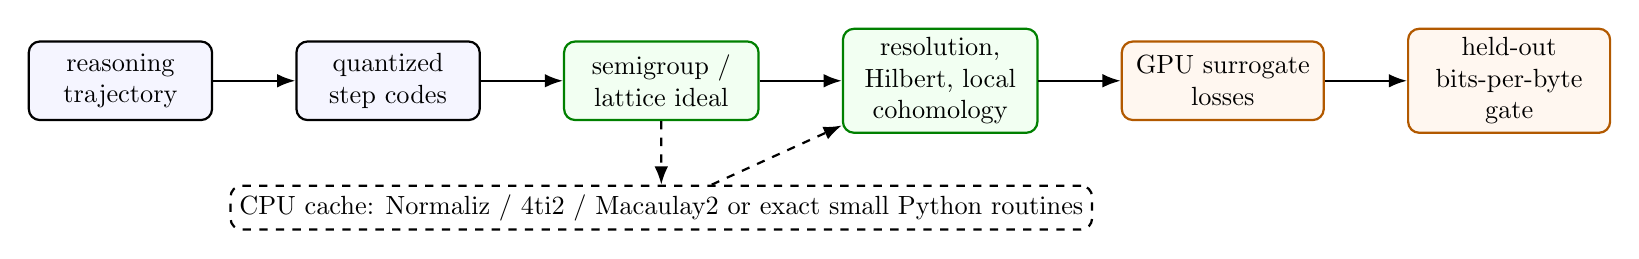
\begin{tikzpicture}[node distance=1.1cm,>=Latex,thick,scale=0.95, every node/.style={transform shape}]
\tikzstyle{box}=[rounded corners,draw,align=center,minimum width=2.45cm,minimum height=1.05cm,fill=blue!4]
\tikzstyle{gbox}=[rounded corners,draw=green!50!black,align=center,minimum width=2.6cm,minimum height=1.05cm,fill=green!5]
\tikzstyle{obox}=[rounded corners,draw=orange!70!black,align=center,minimum width=2.7cm,minimum height=1.05cm,fill=orange!6]
\node[box] (traj) {reasoning\\trajectory};
\node[box,right=of traj] (quant) {quantized\\step codes};
\node[gbox,right=of quant] (alg) {semigroup /\\lattice ideal};
\node[gbox,right=of alg] (cert) {resolution,\\Hilbert, local\\cohomology};
\node[obox,right=of cert] (loss) {GPU surrogate\\losses};
\node[obox,right=of loss] (gate) {held-out\\bits-per-byte\\gate};
\draw[->] (traj) -- (quant);
\draw[->] (quant) -- (alg);
\draw[->] (alg) -- (cert);
\draw[->] (cert) -- (loss);
\draw[->] (loss) -- (gate);
\node[align=center,below=.85cm of alg,draw,dashed,rounded corners,fill=white] (cache) {CPU cache: Normaliz / 4ti2 / Macaulay2 or exact small Python routines};
\draw[->,dashed] (alg) -- (cache);
\draw[->,dashed] (cache) -- (cert);
\end{tikzpicture}%
}
\caption{The toric-algebraic training interface.  A hidden reasoning trajectory is quantized into a finite algebraic object.  Exact certificates are computed offline or cached.  Small GPU losses train the model.  Deployment keeps only components that pass held-out bits-per-byte and reasoning gates.}
\end{figure}

\section{Part II of \emph{Combinatorial Commutative Algebra} as a training manual}
Part II, ``Toric Algebra'', has seven chapters.  The following review is intentionally selective: each topic is read through the lens of ToricGT training.

\subsection{Chapter 7: semigroup rings, lattice ideals, Hilbert bases, and initial ideals}
A semigroup ring \(\kk[Q]\) is the algebra with basis \(\{t^a:a\in Q\}\) and multiplication \(t^a t^b=t^{a+b}\).  If \(Q\) is generated by \(a_1,\ldots,a_n\), then the polynomial ring \(S=\kk[x_1,\ldots,x_n]\) maps onto \(\kk[Q]\) by \(x_i\mapsto t^{a_i}\).  The kernel is the lattice ideal
\[
I_L=\langle x^u-x^v: u,v\in \NN^n,\ u-v\in L\rangle,
\]
where \(L\subseteq \ZZ^n\) is the lattice of relations among the generators.  This is the first direct bridge to reasoning models.  If a reasoning trajectory can be described by counts \(u\in\NN^n\) of primitive moves, then a lattice relation \(u-v\in L\) says that two move multisets produce the same abstract reasoning state.  A binomial residual \(x^u-x^v\) is therefore an equivalence residual.

The book emphasizes that affine semigroup structure is polyhedral.  A pointed affine semigroup has a unique finite minimal generating set.  For a rational pointed cone \(C\), Gordan's lemma gives finite generation of \(C\cap A\); its unique minimal generating set is the Hilbert basis.  In machine-learning language, a Hilbert basis is a minimal reusable dictionary for lattice-respecting states.  If the learned step dictionary is larger than the Hilbert basis, the model may be wasting parameters; if it is smaller, it may be missing states and forcing brittle interpolation.

Initial ideals of lattice ideals under weight orders are the algebraic form of degenerating a binomial problem to a monomial one.  For ToricGT this is exactly what a ReLU or tropical head often does: it chooses an active monomial, active predecessor, active face, or active proof obligation by a weight comparison.  Thus initial ideals provide a rigorous language for training curricula that begin with monomial shadows and lift to binomial consistency.

\subsection{Chapter 8: multigradings, K-polynomials, Betti numbers, and multidegrees}
A multigrading by an abelian group \(A\) assigns \(\deg(x_i)=a_i\).  Hilbert series and K-polynomials become multigraded summaries of which states exist at each degree.  In ToricGT, a degree can encode token budget, proof depth, tool permissions, memory source, verifier confidence, behavior corridor, algebraic task type, or GraphCG coordinate bucket.  The K-polynomial is the alternating Euler characteristic of a free resolution; it summarizes a complex without storing every chain group.

A central training lesson is upper semicontinuity: passing to an initial submodule preserves the Hilbert series but can only increase Betti numbers.  This gives a conservative diagnostic.  If the monomial or ReLU-degenerated shadow of a trajectory has large Betti numbers, then the true hidden algebraic object cannot have larger efficiency than the shadow suggests.  The shadow can be used as an inexpensive upper-bound monitor for syzygetic complexity.

Multidegrees are equivariant Chow-class-like invariants.  In ToricGT they can serve as coarse but stable fingerprints of reasoning families.  They are less brittle than exact Betti tables and better aligned with geometric generalization across equivalent embeddings.

\subsection{Chapter 9: syzygies of lattice ideals}
Chapter 9 explains why lattice ideals behave like infinite periodic monomial ideals.  Laurent monomial modules \(M\subseteq \kk[x_1^{\pm1},\ldots,x_n^{\pm1}]\) replace finite monomial staircases by periodic or infinite staircases.  Hull complexes and Scarf complexes then give cellular resolutions.  For a generic Laurent monomial module, the Scarf complex, hull resolution, and minimal free resolution coincide.  For a generic lattice ideal, the minimal free resolution is the image of the Scarf complex.

For ToricGT this is a blueprint for trajectory-memory compression.  Many reasoning trajectories differ by periodic rewrites: commute independent steps, swap equivalent evidence orderings, rotate through a template, or translate along a memory loop.  A lattice-module representation lets the model learn the periodic quotient instead of memorizing every translate.

\subsection{Chapter 10: toric varieties as multigraded quotients}
Chapter 10 explains how multigraded polynomial rings produce toric varieties through abelian group actions, projective quotients, and Cox-like constructions.  For training, the important point is quotienting.  Many nuisance transformations in reasoning should be quotiented out: graph relabeling, synonym choice, tool-call identifier choice, equivalent proof-step order, and benign style variation.  A toric quotient objective trains the hidden representation to preserve the quotient-invariant part while retaining enough local data for decoding.

\subsection{Chapter 11: irreducible and injective resolutions}
Free resolutions describe generators and syzygies.  Injective and irreducible resolutions describe components, supports, and failure modes.  For a model, these are not interchangeable.  A free-resolution objective asks, ``Are the proof obligations generated efficiently?''  An injective/irreducible objective asks, ``Where can the reasoning fail, and what components are responsible?''  Bass numbers are the dual homological invariants to Betti numbers.  In a verifier or hallucination-control setting, Bass-like features are natural classifiers of missing support and irreducible failure components.

\subsection{Chapter 12: Ehrhart polynomials, dualizing complexes, Brion's formula, and short rational functions}
Ehrhart theory counts lattice points in dilates of a polytope.  It therefore counts how many discrete states are available at a budget scale.  In ToricGT, dilating a polytope can mean increasing reasoning length, evidence budget, context window, number of retrieved memories, or number of allowed graph-of-thought branches.  Brion's formula decomposes a lattice-point generating function into vertex contributions; this is a natural retrieval cache design: instead of storing all states, store vertex-cone summaries and reconstruct counts or priors locally.  Short rational generating functions give compact count surrogates useful for bits-per-byte and artifact budgets.

\subsection{Chapter 13: local cohomology}
Local cohomology measures sections supported on a closed set.  It can be computed with Cech complexes; for semigroup rings, toric local cohomology reduces degreewise to cohomology of polyhedral cocomplexes.  This is directly useful for auditing missing reasoning regions.  A model may perform well in ordinary likelihood while having holes: missing evidence combinations, unsupported behavior corridors, or disconnected retrieval regions.  Local cohomology provides a way to detect these holes as homological obstructions rather than as scattered errors.

\subsection{A map from Part II to ToricGT components}
\begin{longtable}{p{0.17\linewidth}p{0.33\linewidth}p{0.40\linewidth}}
\toprule
Book object & Training interpretation & Example ToricGT use \\
\midrule
Semigroup \(Q\) & allowed finite compositions of primitive reasoning moves & trajectory state dictionary, retrieval-key algebra \\
Lattice ideal \(I_L\) & equivalence of move multisets & binomial relation loss; proof-path equivalence \\
Hilbert basis & minimal nonredundant generator dictionary & step-code pruning; low-byte basis selection \\
Initial ideal & ReLU/tropical degeneration & monomial shadow curriculum; active-cell audit \\
K-polynomial & compressed Euler characteristic of a resolution & low-byte signature for trajectory family \\
Multigraded Betti table & distribution of generators and syzygies by degree & reasoning-depth regularity; proof-obligation complexity \\
Scarf complex & minimal generic cellular resolution & sparse certificate for generic trajectory lattice \\
Toric quotient & invariant representation under group action & graph relabeling, style, and tool-ID invariance \\
Injective resolution & component/failure support & hallucination and missing-evidence classifiers \\
Ehrhart series & growth of admissible states with budget & context-length planning and retrieval capacity \\
Brion decomposition & vertex-local generating functions & sparse vector database/retrieval cache \\
Local cohomology & missing support / holes & coverage loss for evidence, tools, and behavior corridors \\
\bottomrule
\end{longtable}

\section{Reasoning trajectories as semigroup, lattice, and module data}
\subsection{Quantized reasoning-step alphabets}
Let \(G_t\) be the graph-of-thought state at step \(t\), including hidden state \(h_t\), active cells, retrieved memories, verifier fields, and behavior coordinates.  A quantizer
\[
q_\phi(G_t,G_{t+1})\in\{1,\ldots,n\}
\]
assigns a primitive move type to the transition.  A completed trajectory \(\tau\) then gives a count vector \(u(\tau)\in\NN^n\), where \(u_i(\tau)\) is the number of times primitive move \(i\) was used.  A step dictionary assigns each primitive move a degree \(a_i\in A\), where \(A\) is an abelian group such as \(\ZZ^d\oplus \ZZ/c_1\oplus\cdots\).  The degree of a trajectory is
\[
\deg(\tau)=\sum_{i=1}^n u_i(\tau)a_i.
\]
The semigroup \(Q=\NN\{a_1,\ldots,a_n\}\subseteq A\) is the set of reachable abstract degrees.

\begin{definition}[Toric trajectory presentation]
A toric trajectory presentation is a tuple
\[
\mathcal{P}=(A, a_1,\ldots,a_n, L, S, I_L),
\]
where \(A\) is an abelian grading group, \(a_i\in A\), \(L=\ker(\ZZ^n\to A)\), \(S=\kk[x_1,\ldots,x_n]\) with \(\deg(x_i)=a_i\), and \(I_L=\langle x^u-x^v:u-v\in L\rangle\).  A trajectory \(\tau\) is represented by \(x^{u(\tau)}\), and two trajectory codes are algebraically equivalent when their difference lies in \(L\).
\end{definition}

\begin{proposition}[Semigroup factorization of trajectory codes]
Let \(\Psi:S\to R\) be a predicted algebra map into a commutative algebra of scalar hidden features, with \(\Psi(x_i)=z_i\).  Then \(\Psi\) factors through \(\kk[Q]\cong S/I_L\) if and only if
\[
\prod_i z_i^{u_i}=\prod_i z_i^{v_i}\quad\text{for every }u-v\in L.
\]
Equivalently, every binomial in \(I_L\) has zero residual under \(\Psi\).
\end{proposition}
\begin{proof}
By the universal property of quotient rings, \(\Psi\) factors through \(S/I_L\) exactly when \(I_L\subseteq\ker\Psi\).  Since \(I_L\) is generated by binomials \(x^u-x^v\) with \(u-v\in L\), this condition is precisely \(\Psi(x^u-x^v)=0\), which is the displayed equality.
\end{proof}

The associated differentiable loss on a finite relation set \(\mathcal{R}\subset L\) is
\[
\mathcal{L}_{\rm binom}=\frac{1}{|\mathcal{R}|}\sum_{(u,v)\in\mathcal{R}}
\left(\sum_i u_i\log(z_i+\epsilon)-\sum_i v_i\log(z_i+\epsilon)\right)^2.
\]
The logarithmic form avoids numerical explosion and converts products into additive constraints.  It is valid when \(z_i\ge 0\), which is natural for soft counts, gates, positive retrieval scores, or exponentiated affine probes.

\subsection{The bits-per-byte gate}
Let \(D=(b_1,\ldots,b_T)\) be a held-out byte stream and \(q_\theta(b_t\mid b_{<t})\) the deployed predictive distribution.  We write
\[
\mathrm{bits\text{-}per\text{-}byte}(q_\theta;D)=
-\frac{1}{T}\sum_{t=1}^T\log_2 q_\theta(b_t\mid b_{<t}).
\]
If an auxiliary certificate family \(C\) costs \(B(C)\) serialized bits at deployment, its net compression utility on a held-out stream is
\[
U(C)=\sum_{t=1}^T \log_2\frac{q_{\theta,C}(b_t\mid b_{<t})}{q_{\theta}(b_t\mid b_{<t})}-B(C).
\]
Training-only certificates have \(B(C)=0\) at deployment but can still be rejected if their distillation worsens the exported score.

\begin{theorem}[Score-first auxiliary criterion]
A deployed auxiliary certificate or head improves the codelength of a held-out byte stream exactly when \(U(C)>0\).  It improves held-out bits-per-byte exactly when
\[
\frac{1}{T}\sum_{t=1}^T \log_2\frac{q_{\theta,C}(b_t\mid b_{<t})}{q_{\theta}(b_t\mid b_{<t})} > \frac{B(C)}{T}.
\]
\end{theorem}
\begin{proof}
The codelength in bits under \(q_\theta\) is \(-\sum_t\log_2 q_\theta(b_t\mid b_{<t})\).  With auxiliary \(C\), the total codelength includes the serialized certificate bits and equals \(B(C)-\sum_t\log_2 q_{\theta,C}(b_t\mid b_{<t})\).  Subtracting the auxiliary codelength from the baseline codelength yields \(U(C)\).  Dividing by \(T\) gives the bits-per-byte condition.
\end{proof}

This elementary theorem is the central engineering constraint of the paper.  A Hilbert basis loss, a Scarf certificate, or a local-cohomology head can be mathematically correct and still useless for compression if it does not shift the predictive distribution enough to pay its byte cost.

\subsection{Reasoning modules and filtered complexes}
For each problem instance \(p\), let \(\mathcal{T}_p\) be a finite set of sampled or teacher trajectories.  The multigraded trajectory module is
\[
M_p=\bigoplus_{\tau\in\mathcal{T}_p}\kk\cdot e_\tau,
\qquad \deg(e_\tau)=\deg(\tau),
\]
with relations generated by known equivalences, verifier-identical endpoints, memory-compatible rewrites, and graph-of-thought merge identities.  A filtered simplicial complex \(\Delta_p(r)\) can be built on primitive factors or trajectory vertices by thresholding coactivation, verifier compatibility, retrieval compatibility, or proof-dependency scores.  The chain complex \(C_\bullet(\Delta_p(r))\) and the module \(M_p\) interact through a degree map: a simplex \(\sigma\) has degree \(\sum_{i\in\sigma}a_i\).  This is the interface between ToricGT II's persistence complexes and Part II's multigraded algebra.

\begin{definition}[Toric algebra certificate]
A toric algebra certificate for a training record is a finite object
\[
\mathcal{C}=(A,Q,L,\mathcal{R},\Delta,\beta,K,\Gamma),
\]
where \(A\) is a grading group, \(Q\) a finitely generated semigroup, \(L\) a lattice of relations, \(\mathcal{R}\subset L\) a finite relation basis or Markov basis fragment, \(\Delta\) a finite cell or simplicial complex, \(\beta\) a Betti/Bass/local-cohomology target slice, \(K\) a K-polynomial or Hilbert-series fragment, and \(\Gamma\) metadata for quotient, saturation, or local-cohomology computations.  The certificate is exact if all listed invariants are computed from the symbolic record, not predicted by the model.
\end{definition}

\section{Toric algebra and ReLU/tropical neural computation}
\subsection{Active regions as weight orders}
A ReLU network is piecewise affine.  A tropical attention head is explicitly piecewise linear: it computes maxima or minima of affine candidate scores.  In either case, a hidden state \(h\) induces a weight vector \(w(h)\) on candidate monomials or primitive moves.  Given a lattice ideal \(I_L\), the initial ideal \(\inw(h)(I_L)\) records which monomial terms dominate the binomial relations at that hidden state.  This is the algebraic shadow of an active ReLU/tropical decision.

\begin{definition}[ReLU-toric chart]
A ReLU-toric chart for a hidden table \(H\in\RR^{m\times d}\) consists of rational affine candidates \(\ell_i(h)=\langle r_i,h\rangle+b_i\), exponent labels \(a_i\in A\), and a relation lattice \(L\subseteq\ZZ^n\).  The chart assigns each token row \(h\) the weight vector \(w_i(h)=\ell_i(h)\), the active set \(\arg\max_i w_i(h)\), and the initial ideal \(\inw(h)(I_L)\).
\end{definition}

\begin{proposition}[Stable active regions give stable monomial shadows]
Fix a finite relation set \(\mathcal{R}\subset L\).  Suppose that for a hidden state \(h\), every binomial \(x^u-x^v\) in \(\mathcal{R}\) has strict weight gap
\[
|\langle w(h),u-v\rangle|\ge \gamma>0.
\]
If \(\|w(h)-w(h')\|_\infty<\gamma/(2D)\), where \(D=\max_{(u,v)\in\mathcal{R}}\|u-v\|_1\), then \(\inw(h)(x^u-x^v)=\inw(h')(x^u-x^v)\) for all \((u,v)\in\mathcal{R}\).
\end{proposition}
\begin{proof}
For any relation \((u,v)\), the change in weight difference is bounded by
\[
|\langle w(h)-w(h'),u-v\rangle|\le \|w(h)-w(h')\|_\infty\|u-v\|_1 < \gamma/2.
\]
Thus the sign of \(\langle w,u-v\rangle\) cannot change, so the leading monomial of each binomial remains the same.
\end{proof}

The proposition motivates a \emph{Groebner-margin loss}
\[
\mathcal{L}_{\rm init\text{-}margin}=\frac{1}{|\mathcal{R}|}\sum_{(u,v)\in\mathcal{R}}\max\{0,\gamma-|\langle w(h),u-v\rangle|\}.
\]
This is not a generic confidence penalty.  It directly increases the stability of the initial monomial shadow of a toric relation set.  For ReLU networks, it discourages tiny, noisy active-region changes that make reasoning brittle.  For tropical attention, it makes dynamic-programming choices inspectable and stable.

\subsection{Why initial degenerations help training}
The book's multigraded theory explains that K-polynomials are preserved under initial degeneration while Betti numbers can only increase.  This suggests a practical curriculum.  Train first on an initial monomial shadow because monomial membership, standard monomial enumeration, squarefree support, and cellular complexes are cheap.  Then lift to binomial consistency once the hidden representation has stable active cells.

\begin{theorem}[Conservative monomial-shadow curriculum]
Let \(M\) be a finitely generated multigraded module over \(S\), and let \(\inw(M)\) be an initial module under a positive weight order.  Suppose a ToricGT probe estimates Betti masses from the monomial shadow \(\inw(M)\).  If the shadow has Betti mass above a threshold \(B\) in degrees outside an allowed region \(\mathcal{D}\), then no flat lift to \(M\) can have larger homological efficiency penalty than the shadow; i.e. the shadow is a conservative upper-bound diagnostic for syzygy complexity.
\end{theorem}
\begin{proof}
The algebraic fact is that passing to an initial module preserves the multigraded Hilbert series but cannot decrease the number of minimal syzygies in any multidegree.  Thus the Betti numbers of \(\inw(M)\) upper bound those of \(M\) degreewise.  Any penalty that is monotone in the offending Betti masses is therefore an upper-bound penalty.  Training against the shadow may over-penalize, but it will not miss a high-complexity shadow that would signal unstable or redundant reasoning.
\end{proof}

\subsection{ReLU network applications}
The ReLU/tropical applications are concrete.
\begin{enumerate}[leftmargin=*]
\item \textbf{Active proof-path audit.}  Each proof choice is a tropical maximum; the initial monomial records the selected predecessor or rule.  Relation margins measure robustness.
\item \textbf{Symbolic dynamic-programming circuits.}  Shortest path, alignment, parsing, and template matching are min-plus circuits; their graph-token implementation can be audited through monomial shadows.
\item \textbf{Reasoning-cell compression.}  Quantized active-cell IDs plus relation margins can replace long explanation traces when the cell ID predicts future tokens.
\item \textbf{Normal-fan curriculum.}  Start with coarse active-cell labels; refine to binomial relation residuals; then train Betti/local-cohomology certificates.
\item \textbf{Adversarial cell smoothing.}  Penalize active-region changes not justified by changes in input graph structure, verifier state, or retrieved evidence.
\end{enumerate}

\section{Catalog of toric-algebraic applications, losses, metrics, techniques, and regularizers}
This section contains twenty-four objectives and techniques.  The first twenty-two are directly grounded in Part II of the book; the last two are connective techniques that combine multiple Part II themes.  Each item is intentionally phrased as an implementable training component: source idea, mathematical formula, intended compression/reasoning mechanism, and reproducibility details.

\subsection{O1. Semigroup trajectory congruence loss}
\paragraph{Part II source.} Chapter 7: semigroup rings and lattice ideals.
\paragraph{Mathematical object and loss.} Given primitive reasoning moves with degrees $a_i$, build $L=\ker(\ZZ^n\to A)$ and a finite relation set $\mathcal R\subset L$.  For positive move scores $z_i(h)$, use $\mathcal L=|\mathcal R|^{-1}\sum_{(u,v)}(\langle u,\log z\rangle-\langle v,\log z\rangle)^2$.
\paragraph{Why it should help ToricGT.} Equivalent proof paths should induce equivalent hidden codes.  This lowers conditional entropy when future tokens depend on the abstract proof state rather than on an arbitrary ordering of independent moves.
\paragraph{Implementation and reproducibility.} Generate relation sets from small integer kernels by Smith normal form or saturation.  Cache relations by task family.  Evaluate on path-equivalence, proof-order, and graph-relabeling splits.  Use the score-first protocol: report held-out bits-per-byte, task accuracy, proof/verifier metrics, retrieval recall, behavior-corridor violations, and exported artifact bytes before and after enabling this component.  If the exact symbolic audit and differentiable surrogate disagree, the component remains audit-only.


\subsection{O2. Saturation-hole normality regularizer}
\paragraph{Part II source.} Chapter 7: affine semigroups, Hilbert bases, saturation.
\paragraph{Mathematical object and loss.} For a learned semigroup $Q=\NN\{a_i\}$ and sampled lattice point $b$, detect $kb\in Q$ while $b\notin Q$.  Penalize the score assigned to unsupported holes by $\mathcal L_{hole}=\E_b \one[kb\in Q, b\notin Q]s_\theta(b)$, or train a classifier for $Q$ versus $Q^{sat}\setminus Q$.
\paragraph{Why it should help ToricGT.} Nonnormal holes are states that appear reachable by scaling but are not actually reachable by primitive moves.  In reasoning, these cause brittle interpolation: the model extrapolates a plausible intermediate proof state that no valid sequence realizes.
\paragraph{Implementation and reproducibility.} Use Normaliz for larger semigroups; for small records solve bounded integer programs.  Ablate on tasks requiring intermediate lemmas and long-context partial plans.  Use the score-first protocol: report held-out bits-per-byte, task accuracy, proof/verifier metrics, retrieval recall, behavior-corridor violations, and exported artifact bytes before and after enabling this component.  If the exact symbolic audit and differentiable surrogate disagree, the component remains audit-only.


\subsection{O3. Hilbert-basis step dictionary pruning}
\paragraph{Part II source.} Chapter 7: unique minimal generators and Hilbert bases.
\paragraph{Mathematical object and loss.} Let $H_Q$ be the Hilbert basis of the cone generated by step degrees.  Penalize primitive moves not used in any Hilbert-basis decomposition and encourage dictionary coverage: $\mathcal L_{HB}=\alpha |D\setminus H_Q|+\beta\sum_{h\in H_Q}\max(0,\gamma-p_\theta(h))$.
\paragraph{Why it should help ToricGT.} A compact generator dictionary improves bits-per-byte by reducing redundant latent categories and making trajectories share codes.  It also improves reasoning by forcing primitive moves to be irreducible obligations rather than arbitrary microsteps.
\paragraph{Implementation and reproducibility.} Run after quantization stabilizes.  Use soft assignments during training; export only the pruned dictionary if it improves validation.  Use the score-first protocol: report held-out bits-per-byte, task accuracy, proof/verifier metrics, retrieval recall, behavior-corridor violations, and exported artifact bytes before and after enabling this component.  If the exact symbolic audit and differentiable surrogate disagree, the component remains audit-only.


\subsection{O4. Groebner-shadow curriculum}
\paragraph{Part II source.} Chapter 7 initial ideals and Chapter 8 degeneration.
\paragraph{Mathematical object and loss.} For each lattice relation $x^u-x^v$, train first on the leading monomial under a sampled weight $w$, then on the full binomial.  Schedule $\lambda_{binom}$ from 0 to 1 after initial-shadow accuracy exceeds a threshold.
\paragraph{Why it should help ToricGT.} Monomial shadows are easier: they are discrete active choices.  Lifting to binomial relations later teaches equivalence.  This matches how ReLU/tropical networks first learn active regions and then learn stable algebra inside those regions.
\paragraph{Implementation and reproducibility.} Record weight vectors, leading terms, and shadow accuracy.  Reject if the lifted relation loss improves synthetic algebra but worsens natural-text bits-per-byte.  Use the score-first protocol: report held-out bits-per-byte, task accuracy, proof/verifier metrics, retrieval recall, behavior-corridor violations, and exported artifact bytes before and after enabling this component.  If the exact symbolic audit and differentiable surrogate disagree, the component remains audit-only.


\subsection{O5. Multigraded K-polynomial trajectory signature}
\paragraph{Part II source.} Chapter 8 Hilbert series and K-polynomials.
\paragraph{Mathematical object and loss.} For a trajectory module $M$, compute or estimate $K(M;t)=\sum_{i,a}(-1)^i\beta_{i,a}t^a$.  Train a small head $\hat K_\theta(\tau)$ with squared or contrastive loss against the exact finite $K$-slice.
\paragraph{Why it should help ToricGT.} The K-polynomial is a small Euler-characteristic code for a complex.  It can be a retrieval key that captures the shape of a proof family without storing every step.
\paragraph{Implementation and reproducibility.} Flatten only degrees appearing in a bounded window.  Use as a teacher for memory retrieval; do not add to final logits unless retrieval lift appears.  Use the score-first protocol: report held-out bits-per-byte, task accuracy, proof/verifier metrics, retrieval recall, behavior-corridor violations, and exported artifact bytes before and after enabling this component.  If the exact symbolic audit and differentiable surrogate disagree, the component remains audit-only.


\subsection{O6. Betti-table reasoning regularity}
\paragraph{Part II source.} Chapter 8 multigraded Betti numbers.
\paragraph{Mathematical object and loss.} Let $\beta_{i,a}$ be target Betti masses for the record's resolution.  Penalize off-pattern syzygies: $\mathcal L_\beta=\sum_{i,a}w_{i,a}|\hat\beta_{i,a}-\beta_{i,a}|^2+\eta\sum_{(i,a)\notin\mathcal D}\hat\beta_{i,a}$.
\paragraph{Why it should help ToricGT.} High off-pattern Betti mass means redundant obligations or tangled dependencies.  Lowering it encourages proofs whose intermediate constraints compose cleanly.
\paragraph{Implementation and reproducibility.} Use exact Macaulay2 for curated algebra records and synthetic small examples.  For non-algebra tasks, train only coarse Betti buckets from filtered complexes.  Use the score-first protocol: report held-out bits-per-byte, task accuracy, proof/verifier metrics, retrieval recall, behavior-corridor violations, and exported artifact bytes before and after enabling this component.  If the exact symbolic audit and differentiable surrogate disagree, the component remains audit-only.


\subsection{O7. Multidegree class matching}
\paragraph{Part II source.} Chapter 8 multidegrees.
\paragraph{Mathematical object and loss.} Compute a multidegree $C(M;t)$ for exact modules or a proxy from occupied cells.  Train $\hat C_\theta$ using cosine or Earth-mover distance over monomial terms.
\paragraph{Why it should help ToricGT.} Multidegrees are coarser than full resolutions and therefore more robust.  They can group families of equivalent reasoning trajectories across rephrasings and graph isomorphisms.
\paragraph{Implementation and reproducibility.} Use for cross-domain retrieval: same multidegree class but different surface tokens should be positive pairs.  Use the score-first protocol: report held-out bits-per-byte, task accuracy, proof/verifier metrics, retrieval recall, behavior-corridor violations, and exported artifact bytes before and after enabling this component.  If the exact symbolic audit and differentiable surrogate disagree, the component remains audit-only.


\subsection{O8. Initial-Betti upper-semicontinuity gate}
\paragraph{Part II source.} Chapter 8 Betti increase under initial ideals.
\paragraph{Mathematical object and loss.} Compute Betti complexity on a monomial initial shadow.  Gate expensive binomial or homological training only if the shadow complexity is below a budget or the task is tagged as needing high complexity.
\paragraph{Why it should help ToricGT.} This prevents the model from wasting capacity on records whose degenerated shadow is already too tangled for the intended small artifact.
\paragraph{Implementation and reproducibility.} Use a cheap monomial-resolution approximation.  Log `shadow Betti budget exceeded' separately from model failure.  Use the score-first protocol: report held-out bits-per-byte, task accuracy, proof/verifier metrics, retrieval recall, behavior-corridor violations, and exported artifact bytes before and after enabling this component.  If the exact symbolic audit and differentiable surrogate disagree, the component remains audit-only.


\subsection{O9. Laurent periodic trajectory module}
\paragraph{Part II source.} Chapter 9 Laurent monomial modules.
\paragraph{Mathematical object and loss.} Model periodic rewrites by a Laurent monomial module $M\subset\kk[x_1^{\pm1},\ldots,x_n^{\pm1}]$.  Train keys invariant under lattice translations $u\mapsto u+\ell$, $\ell\in L$, by contrastive loss $\|k(u)-k(u+\ell)\|^2$.
\paragraph{Why it should help ToricGT.} Many reasoning differences are periodic or commutative.  Quotienting them improves memory reuse and reduces duplicate storage.
\paragraph{Implementation and reproducibility.} Sample lattice translations within a bounded window.  Combine with graph-of-thought merge labels and retrieval positives.  Use the score-first protocol: report held-out bits-per-byte, task accuracy, proof/verifier metrics, retrieval recall, behavior-corridor violations, and exported artifact bytes before and after enabling this component.  If the exact symbolic audit and differentiable surrogate disagree, the component remains audit-only.


\subsection{O10. Hull-resolution trajectory scaffold}
\paragraph{Part II source.} Chapter 9 hull resolutions.
\paragraph{Mathematical object and loss.} Build the hull complex of a Laurent module or finite truncation; use its bounded faces as scaffold labels for trajectory dependencies.  Penalize predicted boundary matrices by $\sum_k\|\hat D_{k-1}\hat D_k\|_F^2$ and optional alignment.
\paragraph{Why it should help ToricGT.} A hull complex supplies a cellular map of syzygies.  For reasoning, this is a graph of dependency cancellations: which intermediate obligations explain away which redundancies.
\paragraph{Implementation and reproducibility.} Use only bounded finite windows.  Hash the cell complex; stream sparse boundary matrices to GPU.  Use the score-first protocol: report held-out bits-per-byte, task accuracy, proof/verifier metrics, retrieval recall, behavior-corridor violations, and exported artifact bytes before and after enabling this component.  If the exact symbolic audit and differentiable surrogate disagree, the component remains audit-only.


\subsection{O11. Scarf-generic minimal certificate}
\paragraph{Part II source.} Chapter 9 genericity and the Scarf complex.
\paragraph{Mathematical object and loss.} When a lattice or module is generic, use the Scarf complex as the minimal certificate.  Train a Scarf-face predictor and penalize nonunique labels that destroy Scarf minimality.
\paragraph{Why it should help ToricGT.} Minimal certificates are ideal for compression: no redundant cells, no unnecessary syzygies.  This creates compact trajectory signatures.
\paragraph{Implementation and reproducibility.} Add small random rational perturbations to create generic synthetic curricula; keep exact nongeneric cases for robustness tests.  Use the score-first protocol: report held-out bits-per-byte, task accuracy, proof/verifier metrics, retrieval recall, behavior-corridor violations, and exported artifact bytes before and after enabling this component.  If the exact symbolic audit and differentiable surrogate disagree, the component remains audit-only.


\subsection{O12. Lawrence-lift squarefree augmentation}
\paragraph{Part II source.} Chapter 9 Lawrence ideals.
\paragraph{Mathematical object and loss.} Lift relations $u-v\in L$ to $(u-v,v-u)$ in doubled variables and use squarefree initial ideals as augmented contrastive tasks.
\paragraph{Why it should help ToricGT.} Doubled variables separate positive and negative evidence.  Squarefree shadows connect toric relations to simplicial complexes, making them useful for filtered-persistence supervision.
\paragraph{Implementation and reproducibility.} Use for retrieval records with source/target edges or accepted/rejected proof moves.  Avoid storing doubled variables at deployment unless they compress.  Use the score-first protocol: report held-out bits-per-byte, task accuracy, proof/verifier metrics, retrieval recall, behavior-corridor violations, and exported artifact bytes before and after enabling this component.  If the exact symbolic audit and differentiable surrogate disagree, the component remains audit-only.


\subsection{O13. Toric quotient invariance head}
\paragraph{Part II source.} Chapter 10 toric varieties and quotients.
\paragraph{Mathematical object and loss.} Let an abelian group $G$ act on latent coordinates by characters.  Penalize variation of invariant heads under sampled group actions: $\mathcal L_{quot}=\E_g\|f(h)-f(g\cdot h)\|^2$ while preserving equivariant side channels.
\paragraph{Why it should help ToricGT.} Reasoning should ignore nuisance symmetries but preserve task-relevant equivariant information.  Quotient losses separate the two.
\paragraph{Implementation and reproducibility.} Apply to graph relabeling, tool-ID renaming, formatting style, and commuting independent proof steps.  Use the score-first protocol: report held-out bits-per-byte, task accuracy, proof/verifier metrics, retrieval recall, behavior-corridor violations, and exported artifact bytes before and after enabling this component.  If the exact symbolic audit and differentiable surrogate disagree, the component remains audit-only.


\subsection{O14. Cox-style semistable routing window}
\paragraph{Part II source.} Chapter 10 projective quotients.
\paragraph{Mathematical object and loss.} Assign modules to multidegrees and allow an expert or retrieval cell only if the current state is semistable for the chosen degree window.  Penalize routing mass outside the semistable set.
\paragraph{Why it should help ToricGT.} This prevents experts from firing in contexts where their algebraic assumptions are invalid.  It improves reliability and behavior control.
\paragraph{Implementation and reproducibility.} Implement as a learned boolean mask with exact symbolic audits on synthetic quotient examples.  Use the score-first protocol: report held-out bits-per-byte, task accuracy, proof/verifier metrics, retrieval recall, behavior-corridor violations, and exported artifact bytes before and after enabling this component.  If the exact symbolic audit and differentiable surrogate disagree, the component remains audit-only.


\subsection{O15. Irreducible-component hallucination barrier}
\paragraph{Part II source.} Chapter 11 irreducible resolutions.
\paragraph{Mathematical object and loss.} From an evidence semigroup ideal $I$, compute irreducible components $I=\cap_F I_F$.  Penalize answer states that require evidence from mutually incompatible components.
\paragraph{Why it should help ToricGT.} Hallucination often arises by combining fragments that do not share support.  Irreducible components are a precise support decomposition.
\paragraph{Implementation and reproducibility.} Use for retrieval-grounded QA: each evidence span has component labels; final claims must land in a compatible intersection.  Use the score-first protocol: report held-out bits-per-byte, task accuracy, proof/verifier metrics, retrieval recall, behavior-corridor violations, and exported artifact bytes before and after enabling this component.  If the exact symbolic audit and differentiable surrogate disagree, the component remains audit-only.


\subsection{O16. Bass-number failure-mode classifier}
\paragraph{Part II source.} Chapter 11 injective resolutions and Bass numbers.
\paragraph{Mathematical object and loss.} Train a classifier to predict Bass-like component counts $\mu^j_{F,a}$ from hidden states.  Use high Bass degree as a warning for missing support or late-stage failure.
\paragraph{Why it should help ToricGT.} Betti numbers detect generators and syzygies; Bass numbers detect where failures live.  This is useful for abstention, clarification, and verifier routing.
\paragraph{Implementation and reproducibility.} Approximate with component labels for non-algebra records; use exact injective resolutions for small monomial and semigroup examples.  Use the score-first protocol: report held-out bits-per-byte, task accuracy, proof/verifier metrics, retrieval recall, behavior-corridor violations, and exported artifact bytes before and after enabling this component.  If the exact symbolic audit and differentiable surrogate disagree, the component remains audit-only.


\subsection{O17. Dualizing-complex interior evidence prior}
\paragraph{Part II source.} Chapter 12 dualizing complexes.
\paragraph{Mathematical object and loss.} For saturated semigroups, train the model to assign high confidence only to states in the relative interior of the evidence cone; boundary states get uncertainty or request-more-evidence penalties.
\paragraph{Why it should help ToricGT.} Interior states are supported by enough independent evidence directions.  Boundary states often lack hypotheses and should not produce overconfident answers.
\paragraph{Implementation and reproducibility.} Estimate interior membership by linear inequalities.  Couple to tone/personality control: boundary states should sound cautious.  Use the score-first protocol: report held-out bits-per-byte, task accuracy, proof/verifier metrics, retrieval recall, behavior-corridor violations, and exported artifact bytes before and after enabling this component.  If the exact symbolic audit and differentiable surrogate disagree, the component remains audit-only.


\subsection{O18. Ehrhart context-growth law}
\paragraph{Part II source.} Chapter 12 Ehrhart polynomials.
\paragraph{Mathematical object and loss.} Fit the number of admissible reasoning states at budget $m$ to an Ehrhart-like polynomial.  Penalize predicted state counts that violate the learned growth law.
\paragraph{Why it should help ToricGT.} Long-context reasoning needs budget planning.  If admissible states grow polynomially in a structured family, the model should allocate retrieval and branch budget according to that law.
\paragraph{Implementation and reproducibility.} Measure graph-of-thought branch counts at multiple budgets.  Use for stopping-time policies and context-window allocation.  Use the score-first protocol: report held-out bits-per-byte, task accuracy, proof/verifier metrics, retrieval recall, behavior-corridor violations, and exported artifact bytes before and after enabling this component.  If the exact symbolic audit and differentiable surrogate disagree, the component remains audit-only.


\subsection{O19. Brion vertex-cone retrieval cache}
\paragraph{Part II source.} Chapter 12 Brion's formula.
\paragraph{Mathematical object and loss.} Decompose a state polytope into vertex-local cone summaries.  Retrieval score is a mixture over vertex caches: $r(q,m)=\max_v \{r_v(q,m)-c_v\}$ or a softmax variant.
\paragraph{Why it should help ToricGT.} A vertex-cone cache stores local generating functions instead of every state.  This is a principled compression of knowledge-graph neighborhoods and proof-state families.
\paragraph{Implementation and reproducibility.} Index memory by vertex IDs and tangent-cone features.  Evaluate recall at fixed byte budget.  Use the score-first protocol: report held-out bits-per-byte, task accuracy, proof/verifier metrics, retrieval recall, behavior-corridor violations, and exported artifact bytes before and after enabling this component.  If the exact symbolic audit and differentiable surrogate disagree, the component remains audit-only.


\subsection{O20. Short rational generating-function code}
\paragraph{Part II source.} Chapter 12 short rational generating functions.
\paragraph{Mathematical object and loss.} Encode families of reachable states by rational functions $\sum_b c_b t^b=P(t)/\prod_j(1-t^{a_j})$ and distill coefficients or evaluations into a retrieval head.
\paragraph{Why it should help ToricGT.} This turns many discrete states into a compact algebraic code, directly serving compression and bits-per-byte constraints.
\paragraph{Implementation and reproducibility.} Use bounded denominators and exact integer arithmetic during certificate generation; distill to real-valued probes.  Use the score-first protocol: report held-out bits-per-byte, task accuracy, proof/verifier metrics, retrieval recall, behavior-corridor violations, and exported artifact bytes before and after enabling this component.  If the exact symbolic audit and differentiable surrogate disagree, the component remains audit-only.


\subsection{O21. Cech-support local-cohomology loss}
\paragraph{Part II source.} Chapter 13 Cech complexes.
\paragraph{Mathematical object and loss.} For an evidence ideal $I=\langle m_1,\ldots,m_r\rangle$, build the Cech complex and penalize hidden states with high predicted unsupported cohomology in low degrees.
\paragraph{Why it should help ToricGT.} Local cohomology detects information supported only on missing or forbidden loci.  In reasoning, this flags answers relying on unsupported intersections of tools or memories.
\paragraph{Implementation and reproducibility.} Use differentiable cochain maps for small $r$; for large records use sampled supports.  Use the score-first protocol: report held-out bits-per-byte, task accuracy, proof/verifier metrics, retrieval recall, behavior-corridor violations, and exported artifact bytes before and after enabling this component.  If the exact symbolic audit and differentiable surrogate disagree, the component remains audit-only.


\subsection{O22. Toric local cohomology coverage audit}
\paragraph{Part II source.} Chapter 13 toric local cohomology.
\paragraph{Mathematical object and loss.} For degree $b$, compute the cocomplex $\nabla_Q(b)$ and its reduced homology.  Train a coverage head to predict whether $H^i(\nabla_Q(b))$ is nonzero.
\paragraph{Why it should help ToricGT.} Nonzero local cohomology marks holes in semigroup support.  Coverage heads can route the model to retrieve more evidence, ask clarification, or lower confidence.
\paragraph{Implementation and reproducibility.} Convert memory/reasoning states to degrees; compute cocomplexes for small cones; use synthetic holes as adversarial tests.  Use the score-first protocol: report held-out bits-per-byte, task accuracy, proof/verifier metrics, retrieval recall, behavior-corridor violations, and exported artifact bytes before and after enabling this component.  If the exact symbolic audit and differentiable surrogate disagree, the component remains audit-only.


\subsection{O23. Cohen-Macaulay reasoning-depth objective}
\paragraph{Part II source.} Chapter 13 Cohen-Macaulay conditions.
\paragraph{Mathematical object and loss.} Use vanishing patterns of local cohomology or regular-sequence tests as a depth criterion.  Penalize reasoning modules whose low-degree cohomology persists outside expected failure slices.
\paragraph{Why it should help ToricGT.} Cohen-Macaulayness is a strong no-hidden-hole condition.  As a model objective, its proxy encourages robust coverage over all necessary reasoning dimensions.
\paragraph{Implementation and reproducibility.} Use as audit first; train only if the proxy correlates with held-out proof success and bits-per-byte.  Use the score-first protocol: report held-out bits-per-byte, task accuracy, proof/verifier metrics, retrieval recall, behavior-corridor violations, and exported artifact bytes before and after enabling this component.  If the exact symbolic audit and differentiable surrogate disagree, the component remains audit-only.


\subsection{O24. Universal grading discovery}
\paragraph{Part II source.} Chapter 8 universal gradings and lattice ideals.
\paragraph{Mathematical object and loss.} Learn the finest stable grading that makes observed trajectory relations homogeneous.  Penalize relations whose predicted degrees disagree: $\mathcal L_{grade}=\sum_{(u,v)}\|A_\theta u-A_\theta v\|^2$.
\paragraph{Why it should help ToricGT.} A good grading disentangles factors such as evidence, style, tool use, proof depth, and safety.  It improves controllability and retrieval.
\paragraph{Implementation and reproducibility.} Initialize from tags; refine with low-rank integer-like matrices using straight-through rounding.  Use the score-first protocol: report held-out bits-per-byte, task accuracy, proof/verifier metrics, retrieval recall, behavior-corridor violations, and exported artifact bytes before and after enabling this component.  If the exact symbolic audit and differentiable surrogate disagree, the component remains audit-only.


\subsection{O25. Markov-basis negative sampling}
\paragraph{Part II source.} Chapter 7 lattice ideals and integer programming.
\paragraph{Mathematical object and loss.} Use binomial moves from a Markov basis to generate equivalent positive pairs and near-miss negative pairs.  Contrastive loss separates valid lattice moves from invalid moves of similar length.
\paragraph{Why it should help ToricGT.} This trains the model to know which rewrites preserve meaning.  It improves reasoning path search and reduces spurious analogies.
\paragraph{Implementation and reproducibility.} Generate with 4ti2 for curated tasks; for small tasks enumerate bounded kernel moves.  Use the score-first protocol: report held-out bits-per-byte, task accuracy, proof/verifier metrics, retrieval recall, behavior-corridor violations, and exported artifact bytes before and after enabling this component.  If the exact symbolic audit and differentiable surrogate disagree, the component remains audit-only.

\section{Training paradigms derived from Part II}
\subsection{Paradigm A: audit-only algebraic cartography}
Before training any new loss, run the current model on a diagnostic corpus and build toric algebra certificates from hidden trajectories.  Quantize transition types, fit degree maps, compute small relation lattices, estimate semigroups, generate initial ideals under active ReLU/tropical weights, and compute small Betti/K-polynomial/local-cohomology summaries.  No gradient flows through these computations.  The output is a map: which layers and task families already contain recoverable toric structure?

The audit reports:
\begin{enumerate}[leftmargin=*]
\item binomial residuals on known equivalent reasoning paths;
\item semigroup holes and saturation defects;
\item Hilbert-basis coverage of primitive move dictionaries;
\item active initial-ideal stability under perturbations;
\item shadow Betti complexity;
\item Scarf uniqueness and hull-cell sparsity;
\item local-cohomology coverage holes;
\item relation between these diagnostics and held-out bits-per-byte or task errors.
\end{enumerate}

\subsection{Paradigm B: monomial-shadow pretraining and binomial lifting}
This is the safest algebraic curriculum.  Generate records with exact lattice relations, but begin by training only the initial monomial shadows.  The model learns active choices: which proof predecessor, which rewrite, which evidence component, which semigroup generator.  After active margins stabilize, introduce the binomial equality losses.  This mirrors the algebraic fact that initial degeneration preserves Hilbert series while simplifying relations.

\subsection{Paradigm C: ReLU/tropical chart regularization}
For a chosen set of layers, attach low-rank rational probes whose candidate slopes define Newton polytopes and weight orders.  Train for active-cell stability, relation margins, and bend consistency across graph relabelings and equivalent examples.  The probes should be fake-quantized so that any exported component has predictable byte cost.

\subsection{Paradigm D: resolution-shaped graph-of-thought training}
For graph-of-thought trajectories, build a cell complex whose vertices are reasoning states and whose higher cells encode merge compatibility or equivalent decompositions.  Train sparse boundary heads with \(D_{k-1}D_k=0\), Betti profile targets, Scarf/hull labels when available, and local-cohomology coverage labels for missing faces.  Use GFlowNet rewards that favor trajectories with low algebraic residuals only when verifier accuracy and held-out bits-per-byte do not degrade.

\subsection{Paradigm E: quotient and behavior control}
Use toric quotient ideas to separate nuisance variables from behavior-critical variables.  Nuisance transformations include graph relabeling, formatting, tool identifier names, independent step ordering, and benign paraphrase.  Behavior-critical variables include safety, evidence sufficiency, uncertainty, tone, proof rigor, and compliance class.  The quotient head should be invariant to the first group and equivariant or controlled with respect to the second.

\subsection{Paradigm F: retrieval and memory as semigroup modules}
ToricGT III treated MCPs, markdown memory, and knowledge graphs as graph-structured vector databases.  The present paper adds the algebraic layer: memory states live in a semigroup module; equivalent updates differ by lattice translations; local neighborhoods are vertex-cone caches; and missing support is detected by local cohomology.  Retrieval keys can include \((K,\beta,C,\nabla)\)-style signatures in addition to dense embeddings.  A retrieval item is useful when it is close in embedding space and compatible in degree, component support, and resolution signature.

\section{Implementation methodology}
\subsection{Data schema}
Each training record should be convertible into the following JSON-like schema.
\begin{verbatim}
{
  "problem_id": str,
  "tokens": [...],
  "graph": {"nodes": [...], "edges": [...]},
  "trajectory": [step_0, ..., step_T],
  "step_types": [i_0, ..., i_{T-1}],
  "degrees": [[...], ...],
  "relations": [[u, v], ...],
  "filtered_complex": {"simplices": [...], "filtration": [...]},
  "certificates": {
     "semigroup": A_matrix,
     "lattice_kernel": L_basis,
     "hilbert_basis": H,
     "initial_terms": {...},
     "betti_slice": {...},
     "local_cohomology_slice": {...}
  },
  "targets": {"answer": ..., "verifier": ..., "behavior": ...}
}
\end{verbatim}
The schema separates exact certificate generation from differentiable training.  Exact computation can be slow and CPU-bound; it is cached by a content hash of \((A,L,\Delta,\text{task tags})\).  GPU batches receive compact tensors: relation indices, sparse boundary matrices, degree labels, component labels, and target vectors.

\subsection{Certificate generators}
For small examples, pure Python is sufficient.
\begin{enumerate}[leftmargin=*]
\item \textbf{Kernel and lattice basis:} compute Smith normal form or use integer row reduction.  For bounded kernels, enumerate moves \(u-v\) with \(\|u\|_1+\|v\|_1\le D\).
\item \textbf{Semigroup membership:} solve a bounded nonnegative integer feasibility problem.  For tiny cases, dynamic programming over degrees works.
\item \textbf{Hilbert basis:} enumerate indecomposable elements in a bounded cone slice, or call Normaliz for real workloads.
\item \textbf{Initial ideals:} given relation set and weight vector, select leading monomials.
\item \textbf{Free resolutions:} for curated algebra examples, call Macaulay2.  For generic Scarf examples, construct the Scarf complex directly from unique least common multiples or Laurent labels.
\item \textbf{Local cohomology:} construct Cech or Ishida-style complexes for small support ideals; compute homology by sparse linear algebra over a finite field.
\end{enumerate}

\subsection{GPU integration}
A minimal PyTorch interface has three parts.
\begin{verbatim}
class ToricAlgebraCertificate:
    relation_u: LongTensor  # [r, n]
    relation_v: LongTensor  # [r, n]
    degrees: LongTensor     # [n, d]
    boundary: list[SparseTensor]
    betti_target: FloatTensor
    component_labels: LongTensor
    local_cohomology_target: FloatTensor

class ToricAlgebraProbe(nn.Module):
    def forward(self, hidden, cert):
        z = positive_step_scores(hidden)
        binom = binomial_residual(z, cert.relation_u, cert.relation_v)
        beta_hat = betti_head(hidden)
        comp_hat = component_head(hidden)
        local_hat = local_cohomology_head(hidden)
        return binom, beta_hat, comp_hat, local_hat
\end{verbatim}
The expensive symbolic objects never need to be materialized as large dense tensors.  Relation matrices are sparse.  Boundary matrices are sparse.  Betti/local-cohomology targets are small slices.  This matches the ToricGT philosophy: training-only structure, low-rank probes, exact audits, and score-first export.

\subsection{Quantization and artifact accounting}
A toric-algebraic head is exportable only when its compressed codelength is justified.  Low-rank factorization is the default:
\[
W=UV^\top,
\qquad U\in\RR^{m\times r},\quad V\in\RR^{d\times r},\quad r\ll d.
\]
Fake quantization during training estimates the exported behavior.  Every component must report:
\[
B_{\rm comp}=B_{\rm weights}+B_{\rm lookup}+B_{\rm code}+B_{\rm metadata}.
\]
A component survives export only if its held-out log-score lift exceeds \(B_{\rm comp}\) in bits, or if the project is in a research-model mode where a predeclared reasoning metric is allowed to improve without bits-per-byte gain.

\subsection{Reproducible evaluation}
Use clustered splits by algebraic family, not random row splits.  A relation family in training should not reappear with only renamed variables in validation.  Report:
\begin{enumerate}[leftmargin=*]
\item held-out bits-per-byte on ordinary prose and structured graph/proof serializations;
\item exact answer accuracy and verifier agreement;
\item equivariance error under graph relabeling;
\item binomial residual on unseen lattice moves;
\item saturation-hole classification accuracy;
\item Hilbert-basis coverage and generator sparsity;
\item initial-shadow stability under perturbation;
\item Betti/K-polynomial/multidegree prediction error;
\item Scarf/hull certificate precision and recall;
\item local-cohomology coverage error;
\item behavior-corridor violations and calibration.
\end{enumerate}
No metric should be interpreted in isolation.  A model with excellent algebraic diagnostics but worse held-out bits-per-byte is not a better compressed model.  It may still be a useful teacher if it improves proof validity or out-of-distribution algebraic reasoning and distills into a smaller student.

\section{Worked examples}
\subsection{A commuting-proof semigroup}
Suppose a toy proof has three primitive moves: \(x_1\) retrieves a lemma, \(x_2\) applies it, and \(x_3\) formats the conclusion.  If retrieval and formatting commute but applying the lemma must occur after retrieval, the multiset relation might include only
\[
x_1x_3-x_3x_1=0
\]
in a noncommutative trace model, but after abelianization the degree relation says \(e_1+e_3=e_3+e_1\), which is trivial.  This example shows why ToricGT needs typed semigroups: the abelian semigroup captures reusable count structure, while the graph-of-thought DAG captures order constraints.  A useful certificate therefore stores both \(Q\) and a partial order on moves.

\subsection{A binomial relation for equivalent decomposition}
Let primitive moves have degrees
\[
a_1=(1,0),\quad a_2=(0,1),\quad a_3=(1,1).
\]
Then \(a_1+a_2=a_3\), and \(I_L=\langle x_1x_2-x_3\rangle\).  In reasoning terms, doing two elementary steps should match a single macro-step.  A model with positive scores \((z_1,z_2,z_3)\) should satisfy
\[
\log z_1+\log z_2-\log z_3\approx 0.
\]
If not, the hidden state treats macro and micro reasoning inconsistently.  On byte prediction, this inconsistency can raise entropy: after a prefix that admits either decomposition, the model does not confidently predict the same continuation.

\subsection{A saturation hole}
Let \(Q=\NN\{(2,0),(0,2),(1,1)\}\subset\ZZ^2\).  The point \((1,0)\) is not in \(Q\), and no multiple \(k(1,0)\) with odd \(k\) lies in \(Q\), but \(2(1,0)=(2,0)\in Q\).  Thus \((1,0)\) is a saturation hole.  As a reasoning analogy, a model may learn that two copies of a subclaim can be proven but fail to represent a single copy.  Penalizing confidence on such holes encourages valid decomposition at the correct scale.

\subsection{A Scarf certificate for generic relation data}
Consider a small generic lattice ideal whose Scarf complex is minimal.  The training record stores only the faces of the Scarf complex and the signed boundary maps.  The model predicts a boundary \(\hat D\) from hidden states, and the local loss \(\|\hat D_{k-1}\hat D_k\|_F^2\) checks chain-complex consistency.  If the Scarf complex is minimal, every cell is necessary; deleting a cell means the model has lost a required dependency.  This makes Scarf certificates attractive for compact reasoning audits.

\subsection{Local cohomology as evidence-hole detection}
Suppose evidence sources define a semigroup \(Q\) of supported combinations.  A degree \(b\) represents the evidence profile needed for an answer.  If the cocomplex \(\nabla_Q(b)\) has nonzero cohomology, then \(b\) lies in a hole or unsupported support pattern.  The model should either retrieve more evidence, ask a clarifying question, or lower confidence.  This is a sharper signal than a generic uncertainty score because it names the combinatorial source of missing support.

\section{Additional theoretical guarantees}
\begin{theorem}[Lattice-translation invariant retrieval]
Let memory keys be functions \(k:\ZZ^n\to\RR^d\) satisfying \(k(u+\ell)=k(u)\) for all \(\ell\in L\).  Then retrieval scores of the form \(r(u,v)=\langle k(u),k(v)\rangle\) descend to the quotient \(\ZZ^n/L\).  Conversely, any score on \(\ZZ^n/L\) can be lifted to an \(L\)-translation invariant score on \(\ZZ^n\).
\end{theorem}
\begin{proof}
If \(u' = u+\ell\) and \(v'=v+\ell'\), then \(k(u')=k(u)\) and \(k(v')=k(v)\), so \(r(u',v')=r(u,v)\).  Thus the score is well-defined on equivalence classes.  Conversely, given \(\bar r\) on the quotient, define \(r(u,v)=\bar r([u],[v])\).  This is invariant by construction.
\end{proof}

\begin{theorem}[Relation-margin robustness]
Let \(z_i(h)>0\) be positive differentiable scores with \(|\log z_i(h)-\log z_i(h')|\le \epsilon\) for all \(i\).  For a relation \((u,v)\), define
\[
R_{u,v}(h)=\langle u-v,\log z(h)\rangle.
\]
Then \(|R_{u,v}(h)-R_{u,v}(h')|\le \epsilon\|u-v\|_1\).  In particular, if \(|R_{u,v}(h)|>\epsilon\|u-v\|_1\), the sign of the relation residual cannot change under perturbation from \(h\) to \(h'\).
\end{theorem}
\begin{proof}
The bound follows from Holder's inequality:
\[
|\langle u-v,\log z(h)-\log z(h')\rangle|\le \|u-v\|_1\|\log z(h)-\log z(h')\|_\infty\le \epsilon\|u-v\|_1.
\]
The sign statement is immediate.
\end{proof}

\begin{theorem}[Sparse certificate advantage]
Let a certificate \(C\) define a partition of validation contexts into cells \(\mathcal{S}\).  Suppose the deployed model without \(C\) uses distribution \(q_0\), and the model with \(C\) uses the cell-conditional mixture \(q_C(b\mid c)=q_s(b\mid c)\) when \(c\in s\).  If
\[
\sum_{s\in\mathcal S}\sum_{t:c_t\in s}\log_2\frac{q_s(b_t\mid c_t)}{q_0(b_t\mid c_t)}>B(C),
\]
then the certificate improves held-out compression.  If the partition is independent of future validation bytes and computed only from prefixes or fixed side information, the comparison is score-valid.
\end{theorem}
\begin{proof}
The first statement is the score-first auxiliary criterion applied after grouping terms by cell.  The validity statement follows because the cell choice does not depend on the byte being scored or any future byte; therefore it defines a normalized prefix-causal predictive distribution.
\end{proof}

\begin{theorem}[Local-cohomology warning rule]
Let a finite evidence certificate assign a degree \(b\) to a proposed answer and let \(H^i(\nabla_Q(b);\kk)\ne 0\) for some forbidden degree range \(i<d_0\).  Suppose the policy maps nonzero forbidden cohomology to either retrieval, clarification, or low-confidence decoding.  Then the policy cannot output a high-confidence answer on that certificate unless the local-cohomology surrogate is wrong or the warning gate is disabled.
\end{theorem}
\begin{proof}
This is a soundness statement about the finite policy, not a theorem about truth in the world.  The gate condition is a deterministic implication from the computed certificate to the allowed action set.  If the exact certificate has forbidden cohomology, high-confidence answer actions are masked.  Therefore such an answer can occur only when the model uses an incorrect surrogate in place of the exact certificate or the mask is not applied.
\end{proof}

\begin{remark}
The last theorem illustrates the appropriate style of guarantee for learning systems.  The algebra can certify a property of the internal finite record.  It cannot certify that the external world matches the record.  Grounding still requires source verification and data hygiene.
\end{remark}

\section{A concrete experimental plan}
\subsection{Synthetic algebra suite}
Build a suite with increasing difficulty:
\begin{enumerate}[leftmargin=*]
\item small semigroups in \(\ZZ^2\) and \(\ZZ^3\) with known Hilbert bases;
\item saturated versus unsaturated semigroups with labeled holes;
\item lattice ideals from random small matrices and curated nongeneric examples;
\item generic Scarf examples and nongeneric counterexamples;
\item Lawrence lifts with squarefree initial ideals;
\item Ehrhart counting tasks for small polytopes;
\item local-cohomology cocomplex classification tasks.
\end{enumerate}
Every example stores exact certificates.  Splits are by semigroup family and matrix distribution, not by random row.

\subsection{Reasoning suite}
Convert the algebraic objects into reasoning tasks:
\begin{enumerate}[leftmargin=*]
\item proof-path equivalence under commuting independent lemmas;
\item macro-step versus micro-step decomposition;
\item retrieval of a helper proof with same Betti/K signature;
\item detection of missing evidence holes;
\item controlled style: boundary evidence should produce cautious tone;
\item ReLU/tropical dynamic-programming tasks with active initial-ideal labels;
\item graph-of-thought merge consistency under branch recombination.
\end{enumerate}

\subsection{Ablations}
The minimal ablation table is:
\begin{center}
\begin{tabularx}{\linewidth}{p{0.30\linewidth}X}
\toprule
Ablation & Question \\
\midrule
No toric algebra certificates & Does the base ToricGT representation already learn the relation? \\
Only monomial shadows & Are active choices enough without binomial equivalence? \\
Binomial loss without saturation & Are holes responsible for failures? \\
Hilbert-basis pruning disabled & Does dictionary redundancy hurt bits-per-byte? \\
No Betti/K signature in retrieval & Does homological retrieval beat embedding-only retrieval? \\
No local cohomology & Does coverage detection reduce hallucination or overconfidence? \\
No quotient invariance & Are nuisance symmetries leaking into reasoning? \\
Training-only certificates, no export & Is the benefit distillable? \\
Exported low-rank head & Does the compressed head pay for its own byte cost? \\
\bottomrule
\end{tabularx}
\end{center}

\subsection{Stopping rules}
Stop or disable an auxiliary if any of the following occurs:
\begin{enumerate}[leftmargin=*]
\item held-out bits-per-byte worsens beyond the predeclared tolerance on ordinary prose;
\item exact symbolic audits disagree with the differentiable surrogate on a random certificate sample;
\item the auxiliary improves synthetic algebra but harms natural reasoning or behavior calibration;
\item the exported model loses the improvement seen in floating point;
\item the component introduces non-prefix-causal validation dependence.
\end{enumerate}

\subsection{Expected failure modes}
\paragraph{Overfitting algebraic toys.}  The model may learn to solve exact semigroup examples while harming general language modeling.  Use tagged slice metrics and never promote solely on synthetic gains.
\paragraph{Bad quantization of degrees.}  If the hidden step quantizer is unstable, all downstream algebra becomes noise.  Run audit-only quantizer stability tests before algebraic training.
\paragraph{Incorrect finite relation basis.}  A small relation set may miss important equivalences.  Track residuals on held-out relations and use Markov-basis sampling when available.
\paragraph{Surrogate mismatch.}  A neural Betti/local-cohomology head can become a decorative classifier.  Periodically recompute exact certificates and compare.
\paragraph{Behavior overconstraint.}  Algebraic support constraints should not force robotic tone or refusal.  Couple component warnings to calibrated behavior policies, not rigid final text templates.


\section{Expanded theory: why toric algebra can change learning, not only diagnostics}
This section records the mathematical mechanism behind the proposed objectives.  The common pattern is: choose a finite certificate object from Part II of the book, attach it to a bounded reasoning record, prove that the certificate is invariant under an intended equivalence of trajectories, and train a small differentiable probe to predict or respect that certificate.  The probe is useful for a language or graph model only when it changes the conditional distribution assigned to future bytes, tokens, nodes, or proof obligations.  Thus the mathematical invariants below are never promoted merely because they are elegant; they are promoted when they reduce conditional entropy or improve a predeclared reasoning metric under a score-first protocol.

\subsection{A finite toric algebra certificate functor}
Let \(\mathcal R\) be a bounded family of reasoning records.  A record is a tuple
\[
 r=(G,H,\tau,E,V,\mathcal F, y),
\]
where \(G\) is a graph-of-thought, \(H=(h_v)_{v\in V(G)}\) are hidden states, \(\tau\) is a typed edge relation, \(E\) is retrieved evidence, \(V\) is verifier metadata, \(\mathcal F\) is an optional filtered simplicial complex at every reasoning vertex, and \(y\) is the supervised target.  A \emph{Part-II certificate functor} is a map
\[
  \mathsf C: \mathcal R \longrightarrow \mathsf{Cert}_{\rm toric}
\]
whose output consists of a finite subset of the following data:
\[
(Q,L,H_Q,\mathcal B,\operatorname{in}_w I_L,K,\beta,\Delta_{\rm hull},
\Delta_{\rm Scarf},\mathcal I,\Omega_Q^\bullet,\nabla_Q(\cdot)).
\]
Here \(Q\) is a semigroup of discrete reasoning increments, \(L\) is the lattice of trajectory congruences, \(H_Q\) is the minimal semigroup dictionary or Hilbert basis in the saturated case, \(\mathcal B\) is a finite binomial relation set, \(\operatorname{in}_w I_L\) is an initial monomial shadow, \(K\) is a K-polynomial or a low-degree truncation, \(\beta\) is a Betti profile, \(\Delta_{\rm hull}\) and \(\Delta_{\rm Scarf}\) are cellular supports for syzygies, \(\mathcal I\) is an irreducible or primary support decomposition, \(\Omega_Q^\bullet\) is a dualizing or injective complex when available, and \(\nabla_Q(b)\) is the local-cohomology cocomplex in degree \(b\).  Every object in this list is finite after bounded truncation.

\begin{definition}[Certificate-faithful probe]
A probe \(P_\theta\) attached to a ToricGT hidden state is \(\epsilon\)-certificate-faithful on a validation family \(\mathcal V\) if
\[
  \frac{1}{|\mathcal V|}\sum_{r\in\mathcal V} d_{\mathsf C}\big(P_\theta(H(r)),\mathsf C(r)\big)\leq \epsilon,
\]
where \(d_{\mathsf C}\) is an exact certificate metric: Hamming distance for support and initial-ideal labels, Frobenius residual for boundary matrices, edit distance for cellular face posets, Wasserstein distance for multigraded Betti mass, or relative cohomology mismatch for local-cohomology cocomplexes.
\end{definition}

\begin{definition}[Predictive transfer]
A certificate family has positive predictive transfer at artifact cost \(B\) when the exported model \(q_{\theta,B}\) satisfies
\[
  \Delta_{\rm byte}(\mathsf C)=\frac1N\sum_{t=1}^N
  \log_2\frac{q_{0}(b_t\mid b_{<t})}{q_{\theta,B}(b_t\mid b_{<t})}>0,
\]
under strict prefix dependence and after serialized artifact accounting.  For graph reasoning, replace the next byte by the next audited graph symbol, proof step, or verifier-labeled action and report the corresponding cross-entropy lift separately.
\end{definition}

\begin{theorem}[Certificate invariance under trajectory congruence]
Let \(\pi:T\to Q\) map a free monoid of primitive reasoning moves to a commutative semigroup \(Q\).  Suppose two trajectories \(\gamma,\gamma'\in T\) have exponent vectors \(u,v\in\NN^n\) with \(u-v\in L\), where \(L=\ker(\ZZ^n\to \mathsf{gp}(Q))\).  Then every certificate that factors through \(k[Q]\cong \Bbbk[x_1,\ldots,x_n]/I_L\) assigns the same semigroup degree to \(\gamma\) and \(\gamma'\).  In particular, K-polynomial signatures, multigraded Hilbert degrees, semigroup-degree Betti labels, quotient-invariant retrieval keys, and toric quotient heads are invariant under this congruence.
\end{theorem}

\begin{proof}
The congruence \(u-v\in L\) is exactly the relation \(x^u-x^v\in I_L\).  The quotient presentation \(k[Q]\cong S/I_L\) identifies \(x^u\) and \(x^v\) with the same basis element \(t^{\pi(u)}=t^{\pi(v)}\).  Any invariant constructed from the \(Q\)-grading, or from a free resolution of \(S/I_L\) whose basis elements are labeled by \(Q\)-degrees, therefore depends only on the common class of \(u\) and \(v\).  The listed certificates are all functions of the quotient degree or of modules over the quotient ring, so they are unchanged.
\end{proof}

\subsection{Minimum-description interpretation of Hilbert bases}
A central compression use of Hilbert bases is dictionary selection.  Let \(Q=C\cap A\) be pointed and saturated, and let \(H_Q\) be its Hilbert basis.  Suppose a reasoning state is represented by a nonnegative code vector \(z\in\NN^{|D|}\) over a dictionary \(D\subset Q\), with decoded semigroup element \(\sum_i z_i d_i\).  A dictionary is \emph{complete up to radius \(R\)} if every \(q\in Q\) with height \(\omega(q)\le R\) is representable by nonnegative combinations of dictionary elements.

\begin{proposition}[Hilbert-basis necessity]
If \(D\) is complete up to every radius \(R\), then \(H_Q\subseteq D\).  Consequently a deployable dictionary for exact semigroup steps cannot omit a Hilbert-basis element without losing some reachable state.
\end{proposition}

\begin{proof}
Let \(h\in H_Q\).  If \(h\notin D\) and \(D\) generates all of \(Q\), then \(h=\sum_i z_i d_i\) for nonzero \(z\).  Since all \(d_i\in Q\setminus\{0\}\), this expresses \(h\) as a nontrivial semigroup sum, contradicting irreducibility of \(h\).  Therefore every complete dictionary must contain \(h\).  Since \(h\) has finite height, omitting it already breaks completeness at radius \(R=\omega(h)\).
\end{proof}

\begin{corollary}[Pruning rule]
If a learned reasoning-step dictionary contains a code \(d\notin H_Q\) and \(d=h_1+\cdots+h_m\) with \(h_i\in H_Q\), then storing \(d\) is useful only if it shortens runtime or improves prediction enough to pay its artifact byte cost.  It is not needed for exact reachability.
\end{corollary}

This corollary gives a concrete bits-per-byte experiment.  Train one model with the full learned dictionary and another in which composite semigroup moves are replaced by sequences of Hilbert-basis moves plus recurrence.  If the latter preserves validation loss while reducing artifact bytes, the Hilbert-basis representation is preferred.  If the macro-step improves long reasoning enough to compensate for its stored cost, the macro-step is retained as a cached derived generator rather than as a primitive.

\subsection{Initial ideals as ReLU and tropical shadows}
For a lattice ideal \(I_L\subset S\) and a weight \(w\), the initial ideal \(\operatorname{in}_w(I_L)\) records which monomial side of each binomial relation wins under \(w\).  A ReLU or tropical subnetwork similarly selects active affine pieces.  The two notions meet by using a probe that maps a hidden state \(h\) to a weight vector \(w(h)\in\RR^n\).

\begin{definition}[Initial-shadow loss]
Let \(\mathcal B\subset I_L\) be a finite relation set, with \(b_j=x^{u_j}-x^{v_j}\).  Given a hidden state \(h\), set
\[
  s_j(h)=\langle w(h),u_j-v_j\rangle.
\]
If the audited teacher initial side is \(\ell_j\in\{+1,-1,0\}\), where \(0\) means tie or unresolved, define
\[
  \mathcal L_{\rm init}(h)=\sum_{j:\ell_j\ne0} \log(1+\exp(-\ell_j s_j(h)))
  +\lambda_{\rm tie}\sum_{j:\ell_j=0} s_j(h)^2.
\]
\end{definition}

\begin{theorem}[Piecewise-linear stability of initial shadows]
Assume \(\min_j |s_j(h)|\ge \gamma>0\) and \(\|w(h)-w(h')\|_\infty\le \delta\).  If \(\delta\max_j\|u_j-v_j\|_1<\gamma\), then \(h\) and \(h'\) have the same initial side for every relation in \(\mathcal B\).
\end{theorem}

\begin{proof}
For each relation,
\[
 |s_j(h)-s_j(h')|\le \|w(h)-w(h')\|_\infty\|u_j-v_j\|_1
 \le \delta\max_j\|u_j-v_j\|_1<\gamma.
\]
Thus no score can cross zero.  The sign of \(s_j\), and therefore the chosen initial monomial, is unchanged.
\end{proof}

The stability theorem is a direct training rule: margin is not an aesthetic quantity.  It bounds whether a small hidden perturbation changes the algebraic normal form.  For reasoning agents this is useful because a hidden trajectory with low initial-shadow margin is brittle: tiny context changes can flip which proof relation is used, which retrieved fact is dominant, or which tool call is treated as canonical.

\subsection{K-polynomials as compact multi-step signatures}
The K-polynomial appears as an alternating sum over a free resolution.  In training, this supplies a low-byte signature for multi-step reasoning.  Let \(F_\bullet\) be a finite certificate resolution with basis labels \(a_{i,j}\in A\).  Its truncated K-signature is
\[
  K_{\le D}(F_\bullet)=\sum_{i,j: \|a_{i,j}\|\le D}(-1)^i t^{a_{i,j}}.
\]

\begin{proposition}[Additivity under decomposed reasoning]
Suppose a reasoning problem decomposes into two independent certificate modules \(M_1,M_2\) with a short exact sequence
\[
0\to M_1\to M\to M_2\to 0.
\]
Then the exact K-polynomial satisfies \(K(M)=K(M_1)+K(M_2)\).  Therefore a learned K-signature head can be trained by additivity over graph-of-thought branch composition.
\end{proposition}

\begin{proof}
Hilbert series are additive on short exact sequences.  Multiplying by the common denominator defining the K-polynomial preserves additivity.  Equivalently, choose free resolutions and take the Euler characteristic of multigraded free modules; Euler characteristics are additive in exact triangles.
\end{proof}

For ToricGT this gives a branch-merge consistency loss.  If branches \(b_1,b_2\) are independent and merge into \(m\), require
\[
  \mathcal L_{K\text{-merge}}=\left\|\widehat K(m)-\widehat K(b_1)-\widehat K(b_2)\right\|_1.
\]
The loss is computationally cheap because the signature is a sparse vector over degrees.  It is particularly appropriate for long-context settings: a 1--10M token context can contain many proof branches, but the K-signature of each branch can be stored as a small sparse multiset of degrees.

\subsection{Local cohomology as coverage and uncertainty}
Local cohomology measures support failure.  In the training setting, this means it can diagnose when a reasoning trajectory has a hole: a missing evidence region, an uncovered tool permission, an omitted boundary case, or a sparse retrieval neighborhood that should have been filled before giving a confident answer.

\begin{definition}[Coverage cocomplex of a reasoning state]
Let \(Q\) be the semigroup of certified evidence increments and let \(b\in\ZZ^d\) be the target degree of a reasoning state.  Define
\[
 \nabla_Q^{\rm reason}(b)=\{F\subseteq Q\text{ a face-like support class}: b\in Q-F\}.
\]
If an exact semigroup is not available, approximate \(Q-F\) using retrieved evidence cones and active face labels.  The local-cohomology coverage score is
\[
  \mathrm{Hole}_i(b)=\dim \widetilde H_i\big((\nabla_Q^{\rm reason}(b))^\vee;\Bbbk\big).
\]
\end{definition}

\begin{theorem}[Hole penalty is monotone under evidence completion]
Assume adding evidence enlarges the semigroup support from \(Q\) to \(Q'\supseteq Q\) without changing the ambient face poset.  Then \(\nabla_Q^{\rm reason}(b)\subseteq \nabla_{Q'}^{\rm reason}(b)\).  Thus every newly added evidence item can only add cells to the coverage cocomplex.  In particular, a persistent nonzero reduced homology class after evidence completion identifies a structural rather than accidental coverage hole.
\end{theorem}

\begin{proof}
If \(F\) satisfies \(b\in Q-F\), then \(b=q-f\) for some \(q\in Q\) and \(f\in F\).  Since \(Q\subseteq Q'\), the same representation shows \(b\in Q'-F\).  Hence the cocomplex only grows.  Nonzero homology after repeated additions cannot be blamed on an item that was available but omitted; it reflects the topology of the remaining uncovered region or a mismatch between the chosen faces and the target degree.
\end{proof}

This theorem yields a pragmatic behavior policy.  If a high-confidence answer is produced while \(\mathrm{Hole}_i(b)>0\) for some critical \(i\), lower the confidence corridor, ask for clarification, retrieve more evidence, or emit a qualified answer.  The target is not to make the model timid.  The target is to distinguish ordinary uncertainty from topologically structured missing support.

\section{Detailed Part-II-derived objective cards}
The following cards expand the catalog into reproducible research units.  Each card gives the audit object, differentiable surrogate, expected model benefit, and a minimal ablation.  These are intended to be implemented independently; combining them all at once would make attribution impossible.

\paragraph{Card A: lattice-ideal normal-form head.}
Audit object: a finite Groebner or Markov relation table \(\mathcal B\subset I_L\).  Surrogate: predict a canonical representative \(\operatorname{NF}(u)\) of a move exponent vector \(u\).  Loss:
\[
  \mathcal L_{\rm NF}=\mathrm{CE}(\widehat{\operatorname{NF}}(u),\operatorname{NF}(u))
  +\lambda\sum_{x^a-x^b\in\mathcal B}\|z(a)-z(b)\|_2^2 .
\]
Benefit: reduces duplicate hidden states for equivalent proof paths and improves retrieval precision.  Ablation: remove the relation term while keeping the same canonical-representative labels.

\paragraph{Card B: saturation-hole detector.}
Audit object: holes \(Q^{\rm sat}\setminus Q\) in bounded degree.  Surrogate: binary classifier \(p_{\rm hole}(b\mid h)\).  Loss:
\[
 \mathcal L_{\rm hole}= -y_b\log p_{\rm hole}-(1-y_b)\log(1-p_{\rm hole})
 +\lambda y_b\max(0,c(h)-c_{\max})^2,
\]
where \(c(h)\) is confidence.  Benefit: prevents confident extrapolation through missing evidence.  Ablation: keep the classifier but decouple it from confidence and behavior corridors.

\paragraph{Card C: Hilbert-basis macro/micro controller.}
Audit object: decompositions of reachable moves into Hilbert-basis elements.  Surrogate: a controller decides whether to emit a macro move or a sequence of primitives.  Loss:
\[
\mathcal L_{\rm Hctrl}=\mathcal L_{\rm task}+\lambda_{\rm len}\,\mathbb E[T_{\rm steps}]
+\lambda_B B_{\rm macro}-\lambda_{\rm lift}\Delta_{\rm byte}.
\]
Benefit: discovers when storing a reusable macro is worth bytes and when recurrence suffices.  Ablation: force all macro moves off.

\paragraph{Card D: initial-shadow active-region regularizer.}
Audit object: \(\operatorname{in}_w(I_L)\) labels under teacher weights.  Surrogate: hidden-to-weight map \(w_\theta(h)\).  Loss is \(\mathcal L_{\rm init}\) above plus a margin term.  Benefit: aligns ReLU/tropical active regions with algebraic normal forms.  Ablation: randomize relation labels; performance should collapse if the objective is genuinely algebraic.

\paragraph{Card E: Betti sparsity and regularity.}
Audit object: multigraded Betti table \(\beta_{i,a}\).  Surrogate: sparse Betti head.  Loss:
\[
\mathcal L_{\beta}=\mathrm{BCE}(\widehat{\mathrm{supp}\,\beta},\mathrm{supp}\,\beta)
+\lambda\sum_{i,a}\widehat\beta_{i,a}(|a|-i-r_0)_+.
\]
Benefit: biases trajectories toward resolutions with predictable dependency depth.  Ablation: replace Betti labels by total trajectory length labels and compare OOD proof generalization.

\paragraph{Card F: hull-cell path supervision.}
Audit object: cell path in a hull resolution of a Laurent monomial module.  Surrogate: sequence of predicted cell ids.  Loss combines cell CE with adjacency penalties:
\[
\mathcal L_{\rm hullpath}=\sum_t \mathrm{CE}(\hat c_t,c_t)+\lambda\sum_t \mathbf 1[(\hat c_t,\hat c_{t+1})\notin E_{\rm hull}].
\]
Benefit: teaches the model to traverse syzygy geometry rather than treating every proof step as an unrelated token.  Ablation: same number of labels but shuffled cell adjacency.

\paragraph{Card G: Scarf uniqueness probe.}
Audit object: whether an exponent label is unique among least common multiples or lattice-module labels.  Surrogate: uniqueness probability \(p_{\rm unique}\).  Loss:
\[
\mathcal L_{\rm Scarf}=\mathrm{BCE}(p_{\rm unique},y_{\rm unique})+\lambda H(p_{\rm cell}\mid y_{\rm unique}=1).
\]
Benefit: identifies steps whose explanations are canonical and therefore good candidates for memory.  Ablation: retrieve memories by final embedding only.

\paragraph{Card H: Lawrence squarefree lift.}
Audit object: the Lawrence lift \(\Lambda(L)\) and its squarefree initial shadows.  Surrogate: split each feature into positive/negative channels and penalize non-squarefree coactivation.  Loss:
\[
 \mathcal L_{\rm Law}=\sum_i (p_i^+p_i^-)^2+\lambda\mathcal L_{\rm init}^{\Lambda(L)}.
\]
Benefit: gives a safe binary augmentation for ambiguous directions and sign-sensitive reasoning.  Ablation: remove the positive/negative split.

\paragraph{Card I: irreducible support decomposition.}
Audit object: irreducible components of monomial ideals in \(k[Q]\).  Surrogate: support classifier over face-indexed components.  Loss:
\[
\mathcal L_{\rm irr}=\sum_F \mathrm{BCE}(\hat y_F,y_F)+\lambda\,\mathrm{TV}(\hat y,\text{face order}).
\]
Benefit: separates distinct failure modes that ordinary scalar confidence merges.  Ablation: train a single scalar error classifier.

\paragraph{Card J: Bass-warning head.}
Audit object: Bass numbers \(\mu^j_{F,a}(M)\) along faces and degrees.  Surrogate: low-rank face-degree tensor predictor.  Loss:
\[
\mathcal L_{\rm Bass}=\sum_{j,F,a}w_{j,F,a}\left|\hat\mu^j_{F,a}-\mu^j_{F,a}\right|.
\]
Benefit: detects embedded or delayed failure support, especially when a generated proof appears locally valid but has a hidden boundary defect.  Ablation: replace Bass labels by Betti labels to test whether injective-side information is distinct.

\paragraph{Card K: Ehrhart growth regulator.}
Audit object: counted reachable states in dilated polytopes or filtered context windows.  Surrogate: predicted count polynomial or quasi-polynomial.  Loss:
\[
\mathcal L_{\rm Ehr}=\sum_{m\le M}\left|\log(1+\hat E(m))-\log(1+E(m))\right|^2.
\]
Benefit: learns how many states a reasoning process should create as context grows, preventing both underexploration and combinatorial explosion.  Ablation: replace Ehrhart targets by raw token counts.

\paragraph{Card L: Brion vertex-cache allocation.}
Audit object: vertex-cone decomposition of a generating function.  Surrogate: choose which local cache entries to allocate around vertices of the active polytope.  Loss:
\[
\mathcal L_{\rm Brion}=\mathcal L_{\rm pred}+\lambda\sum_v B_v-\eta\sum_v \mathrm{lift}_v,
\]
with byte cost \(B_v\) and measured lift from vertex-local retrieval.  Benefit: compresses long-context retrieval by storing local rational pieces instead of a large flat table.  Ablation: uniform cache allocation.

\paragraph{Card M: Cech and Ishida coverage.}
Audit object: Cech/Ishida complex for support on an ideal or semigroup maximal support.  Surrogate: cochain residual and cohomology-rank head.  Loss:
\[
\mathcal L_{\rm cov}=\sum_i\|\hat d_{i+1}\hat d_i\|_F^2+
ho\sum_i|\widehat{\dim H^i}-\dim H^i|.
\]
Benefit: turns evidence coverage into a chain-complex problem.  Ablation: a heuristic retrieval-count threshold.

\section{Reproducibility appendix: data, code paths, and exact audits}
\subsection{Canonical record format}
Every synthetic or curated record should be serialized as line-delimited JSON with the following minimal schema:
\begin{verbatim}
{
  "id": "semigroup-family/split/hash",
  "prompt": "natural-language or graph task prompt",
  "graph": {"nodes": [...], "edges": [...], "types": [...]},
  "trajectory": [{"move": "x3*x5", "degree": [1,0,2], "hidden_slot": 4}],
  "certificate": {
    "A": [[...]],
    "L_basis": [[...]],
    "relations": [{"u": [...], "v": [...]}],
    "hilbert_basis": [[...]],
    "initial_labels": [...],
    "betti": [{"i": 0, "deg": [...], "value": 1}],
    "cells": {"vertices": [...], "faces": [...]},
    "local_cohomology": [{"degree": [...], "cohomology": [...]}]
  },
  "target": {"answer": "...", "verifier": true, "bytes": 123}
}
\end{verbatim}
The record hash is computed from the exact certificate, not from the surface prompt.  This prevents leakage in which train and validation share the same semigroup under different prose.

\subsection{Exact certificate generation}
Certificate generation is CPU-side.  The default pipeline is:
\begin{enumerate}[leftmargin=*]
\item Sample or load a small integer matrix \(A\) with columns \(a_i\).
\item Compute \(L=\ker_\ZZ(A)\) by Smith normal form.
\item Generate a bounded binomial relation set and saturate by the product of variables when constructing \(I_L\).
\item Compute Hilbert-basis or saturation-hole data for bounded cones using Normaliz, 4ti2, Sage, Macaulay2, or a verified custom routine for small dimensions.
\item Compute initial-shadow labels under sampled weights \(w\).
\item For small examples, compute multigraded Betti tables and cellular supports by Macaulay2; for large examples, store only bounded-degree targets.
\item Construct local-cohomology cocomplexes by enumerating faces and checking membership in \(Q-F\).
\item Serialize sparse tensors in coordinate format and cache by SHA256.
\end{enumerate}
No symbolic computation should run inside the GPU training step.  The GPU receives dense hidden states, sparse boundary matrices, integer labels, and compressed target vectors.

\subsection{Deterministic validation and leakage control}
The validation protocol must be score-first.  It must also be algebra-split.  A split by random examples is insufficient because many different prompts can encode the same lattice ideal or the same semigroup holes.  Use the following split keys:
\[
\mathrm{split\_key}=\mathrm{hash}\big(\operatorname{SNF}(A),\operatorname{Hilb}(Q)_{\le R},\mathrm{relation\ support},\mathrm{family\ tag}\big).
\]
All records with the same key go to the same split.  For curated reasoning data, add a text-source key and an answer-template key.  Report results on synthetic algebra, translated natural language, graph JSON, proof text, and ordinary prose separately.

\subsection{Recommended hyperparameters}
A conservative first run should use tiny weights:
\[
\lambda_{\rm init}=10^{-4},\quad
\lambda_{\beta}=10^{-4},\quad
\lambda_{\rm hole}=10^{-4},\quad
\lambda_{\rm cov}=10^{-5},\quad
\lambda_{\rm quotient}=10^{-4}.
\]
After probe-only training reaches high certificate accuracy, increase only one family at a time.  The activation order should be
\[
\begin{aligned}
&\text{initial shadows}\to\text{semigroup congruence}\to\text{Hilbert basis}\to\text{Betti/K signatures}\\
&\to\text{Scarf/hull}\to\text{local cohomology}\to\text{dualizing/Bass}.
\end{aligned}
\]
This ordering reflects numerical conditioning.  Initial shadows and congruence labels are local.  Local cohomology and Bass warnings are higher-order support objects and should not be enabled before the representation has stable lower-order structure.

\subsection{Minimal open-source reproduction}
A minimal reproduction can be done without building all of ToricGT:
\begin{enumerate}[leftmargin=*]
\item Train a small graph-token Transformer on graph-labeled semigroup normal-form tasks.
\item Add the lattice-ideal normal-form head and initial-shadow loss.
\item Add Hilbert-basis dictionary pruning.
\item Add a retrieval table keyed by K-signatures and compare against embedding-only retrieval.
\item Evaluate on held-out semigroup families and natural-language explanations of the same tasks.
\item Export an int8 low-rank probe version and report bits-per-byte, exact answer accuracy, and artifact bytes.
\end{enumerate}
This ablation is intentionally narrow.  It can validate the central claim--that toric algebra certificates improve reasoning or compression--before adding Scarf complexes, local cohomology, or behavior corridors.

\subsection{Reporting checklist}
Every experiment should report:
\begin{enumerate}[leftmargin=*]
\item base validation bits-per-byte and tagged-slice bits-per-byte;
\item exported artifact bytes, not just parameter count;
\item exact certificate accuracy on a random audit sample;
\item relation residual on held-out binomials;
\item Hilbert-basis coverage and dictionary byte cost;
\item Betti/K retrieval lift;
\item local-cohomology false-positive and false-negative rates;
\item proof or graph exact-match accuracy;
\item behavior calibration when coverage holes are present;
\item three-seed confidence intervals or matched-checkpoint comparisons.
\end{enumerate}
A component should be called successful only when the relevant target metric improves without a statistically meaningful regression in ordinary prose bits-per-byte, unless the experiment is explicitly a research-only graph-reasoning model rather than a compressed language model.

\section{Wild-card research directions}
\subsection{Toric algebra for mixture-of-experts routing}
A Soft-MoE router can be treated as a semigroup action on expert usage counts.  Let \(q_t\in\NN^E\) record expert counts along a trajectory and let \(L_{\rm route}\) identify count vectors that lead to equivalent outputs.  The routing toric ideal \(I_{L_{\rm route}}\) gives binomial constraints on routes.  A low-rank router can be regularized by
\[
\mathcal L_{\rm route-toric}=\sum_{u-v\in\mathcal B_{\rm route}}
\left|\log p(u\mid h)-\log p(v\mid h)\right|^2,
\]
where \(p(u\mid h)\) is the probability of a route count.  This can reduce mode collapse by identifying routes that are algebraically equivalent while still allowing specialization when equivalence fails.  The export decision is simple: store no extra expert unless its route class improves quality per byte.

\subsection{Semigroup-valued curriculum scheduling}
Training curricula often use ad hoc difficulty scores.  A toric algebra curriculum uses semigroup height, saturation depth, projective dimension, and local-cohomology complexity.  Define
\[
  d_{\rm alg}(r)=\alpha\omega(q_r)+\beta\operatorname{pd}(I_{L_r})+
ho\#(Q_r^{\rm sat}\setminus Q_r)_{\le R}+\eta\sum_i\dim H^i_{\mathfrak m}(k[Q_r])_{b_r}.
\]
Then sample records with probability proportional to \(\exp(-d_{\rm alg}/T_s)\), annealing \(T_s\).  This introduces hard algebraic cases gradually while preserving exact difficulty labels.

\subsection{Universal grading discovery for hidden features}
Part II emphasizes that a lattice ideal has a universal grading by \(\ZZ^n/L\).  For hidden states, one can learn the finest quotient of feature directions under which observed relation residuals are homogeneous.  Given relation differences \(r_j=u_j-v_j\), learn a projection \(P\) such that \(Pr_j\approx0\) for true relations and \(Pr_j\not\approx0\) for false relations:
\[
\mathcal L_{\rm univ}=\sum_{j\in \mathcal R^+}\|Pr_j\|_2^2-	au\sum_{j\in\mathcal R^-}\min(\|Pr_j\|_2^2,m)+\lambda\|PP^T-I\|_F^2.
\]
The rows of \(P\) become learned grading axes.  If they align with GraphCG axes, the model has discovered a quotient structure rather than memorizing individual tasks.

\subsection{Canonical-module evidence priors}
For normal semigroup rings, the canonical module is controlled by interior degrees.  In reasoning, interior degrees correspond to states with enough independent evidence to be away from boundary ambiguity.  A canonical-module prior increases probability mass on answer states whose evidence degree lies in a learned interior cone and decreases overconfident answers on boundary states:
\[
\mathcal L_{\omega}= -\log p(y\mid h)+\lambda\mathbf 1[b\notin\operatorname{relint}(C)]\max(0,c(h)-c_{\partial})^2.
\]
This is a mathematically principled version of ``be more cautious near the boundary of available evidence.''

\subsection{Multigraded Hilbert-scheme view of representation drift}
Across training, the set of hidden relations satisfied by a layer changes.  Treat each checkpoint as a point in an approximate multigraded Hilbert scheme of relation ideals.  A drift metric can be defined by comparing Hilbert functions of the hidden relation ideal:
\[
D_{\rm Hilb}(\theta_s,\theta_t)=\sum_{a\in A_{\le R}}\left|\dim(S/I_{\theta_s})_a-\dim(S/I_{\theta_t})_a\right|.
\]
Large drift late in training signals that the representation is changing its quotient structure and may invalidate cached probes.  This gives a principled checkpoint-triage metric.

\subsection{Integer-programming certificates as tool-use supervision}
The lattice-ideal and Hilbert-basis material is tightly connected to integer programming.  For tool-using agents, a tool-call plan can be treated as a feasible integer point.  A certificate that a plan is irreducible, saturated, or equivalent to another plan becomes a compact supervision target.  Instead of training only on final tool outputs, train on plan normal forms and irreducible decompositions.  This can reduce wasted calls and improve compliance because forbidden tool combinations become monomial nonfaces or semigroup holes.


\section{Conclusion}
Part II of \emph{Combinatorial Commutative Algebra} offers a surprisingly direct training language for ToricGT.  Semigroup rings encode reachable reasoning states; lattice ideals encode equivalences of trajectories; Hilbert bases give minimal dictionaries; initial ideals match ReLU/tropical active shadows; K-polynomials and multidegrees give compact signatures; Betti numbers and Scarf/hull complexes describe dependency structure; toric quotients train invariance; injective resolutions and Bass numbers classify failure support; Ehrhart and Brion theory compress state counts; and local cohomology detects holes.

The primary goal remains model improvement.  The mathematical objects are not decorations.  They are useful only when they reduce held-out bits-per-byte, improve proof and graph reasoning, increase retrieval precision, improve behavior controllability, or provide reliable audits that enable safer training.  The most promising immediate experiments are conservative: audit first, train low-rank probes second, enable monomial shadows before binomial lifts, use exact small certificates, cache aggressively, and export nothing unless the bits-per-byte gate or a predeclared reasoning gate passes.

The larger research program is to make hidden reasoning less shapeless.  A trajectory should have algebraic coordinates, support, quotients, generators, syzygies, and holes.  When those objects are finite and auditable, they can be used to train better reasoning agents without requiring the deployed agent to carry the full machinery of a computer-algebra system.

\begin{thebibliography}{99}
\bibitem{MillerSturmfels2005} Ezra Miller and Bernd Sturmfels. \emph{Combinatorial Commutative Algebra}. Graduate Texts in Mathematics 227. Springer, 2005.
\bibitem{CoxLittleSchenck2011} David Cox, John Little, and Hal Schenck. \emph{Toric Varieties}. American Mathematical Society, 2011.
\bibitem{Sturmfels1996} Bernd Sturmfels. \emph{Groebner Bases and Convex Polytopes}. American Mathematical Society, 1996.
\bibitem{BayerSturmfels1998} Dave Bayer and Bernd Sturmfels. Cellular resolutions of monomial modules. \emph{Journal fuer die reine und angewandte Mathematik}, 1998.
\bibitem{PeevaSturmfels1998} Irena Peeva and Bernd Sturmfels. Generic lattice ideals. \emph{Journal of the American Mathematical Society}, 1998.
\bibitem{BrunsGubeladze} Winfried Bruns and Joseph Gubeladze. \emph{Polytopes, Rings, and K-Theory}. Springer, 2009.
\bibitem{ToricGT} Amelie Schreiber. \emph{ToricGT with Toric BGG Supervision: Graph-Token Reasoning, Hypertoric Category O, and Bits-per-byte-Constrained Training}. Manuscript, 2026.
\end{thebibliography}
\end{document}
